\documentclass[12pt,twoside]{report} 
\usepackage[utf8]{inputenc}
\usepackage{graphicx}

\usepackage{enumitem}
\usepackage[spanish]{babel}
\usepackage{float}
\usepackage{caption}
\usepackage[sorting=none, style=numeric]{biblatex} 
\usepackage{hyperref}
\usepackage{amsmath}
\usepackage{array}
\usepackage{pdfpages}
\bibliography{referencias}

\setcounter{secnumdepth}{3}
\renewcommand\spanishtablename{Tabla}
%%%%%%%%%%%%%%% DISEÑO %%%%%%%%%%%%%%%%%%%%%
\usepackage[a4paper, top=25mm, margin=30mm]{geometry}
\usepackage{fancyhdr}
\pagestyle{fancy}
\fancyhead{}
\renewcommand{\headrulewidth}{0pt}
\fancyfoot{}
\fancyfoot[LE,RO]{\thepage}

\usepackage{etoolbox}
\patchcmd{\chapter}{\thispagestyle{plain}}{\thispagestyle{fancy}}{}{}

%%%%%%%%%%%%%%%%%%%%%%%%%%%%%%%%%%%%%%%%%%%%%


\begin{document}

\begin{titlepage}
    \centering
    
\includegraphics[width=0.8\textwidth]{img/universidad-valladolid-uva.png}\par\vspace{0.5cm}
    {\Large \bfseries FACULTAD DE CIENCIAS\par}
    \vspace{2.5cm}
    {\Large \bfseries TRABAJO FIN DE GRADO\par}
    \vspace{0.5cm}
    {\Large \bfseries Grado en Estadística\par}
    \vspace{0.5cm}
    {\Large\bfseries Librería de muestreo con R: samplingR \par}
    \vspace{4cm}
    
    {\Large \bfseries Autor:\\ D. Javier Estévez Asensio\par}
    {\Large \bfseries Tutores: \\D. Alfonso Gordaliza Ramos, \\ D. Francisco Rodríguez Redondo\par}
    \vspace{0.5cm}
    {\Large \bfseries Año 2023\par}

\end{titlepage}

\newpage
\pagenumbering{Roman}
\setcounter{page}{1}
\chapter*{Abstract}
El muestreo estadístico es una técnica usada en multitud de ámbitos, desde el empresarial hasta el sanitario o el político, permitiendo obtener de forma eficiente y económica información sobre una población completa para realizar una toma de decisiones.\\

En este trabajo, se ha creado una librería de funciones relacionadas con el muestreo estadístico en el programa de software libre R con el objetivo de subirlo al repositorio oficial \textit{CRAN} \cite{CRAN} y ampliar las funcionalidades que ofrecen otras librerías ya publicadas con temática similar. \\\\\\\\

Statistical sampling is a technique used in a multitude of fields, from business to healthcare and politics, allowing for efficient and cost-effective gathering of information on a complete population to aid in decision-making.\\

A library of statistical sampling related functions  has been developed on R free software program with the goal of uploading it to the \textit{Comprehensive R Archive Network (CRAN)} \cite{CRAN} to extend the functionalities offered by other similarly themed libraries already published on it.

\chapter*{Agradecimientos}

Agradezco a mi familia, por brindarme una educación completa y apoyarme desde el primer día hasta el último.\\

A Francisco, por dejarlo todo para ayudarme siempre que lo he necesitado.\\

Y por último, me gustaría agradecer a la promoción 2018/2023 de InDat por unos años maravillosos junto a ellos.

\newpage
\renewcommand*\contentsname{Tabla de contenidos}
\tableofcontents
\newpage

\listoffigures
\newpage

\renewcommand{\listtablename}{Índice de tablas}
\listoftables
\newpage



\pagenumbering{arabic}
\setcounter{page}{1}

\chapter{Introducción}
Para multitud de análisis económicos, demoscópicos, sociosanitarios, etc., resulta de interés conocer el valor de determinados parámetros poblacionales (medias, proporciones, totales, ...), que comúnmente son desconocidos. Ya sea el salario promedio de las familias españolas o el total de accidentes en el sector de la construcción en un determinado territorio, es necesario invertir recursos en realizar un estudio para poder hacer el análisis de los datos de interés en busca de información útil.\\

El muestreo permite realizar un análisis sobre una subpoblación o muestra de la población objetivo a estudiar, obteniendo estimadores que se aproximen al valor real que se conseguiría al realizar el estudio sobre la población completa, con el aliciente de hacerlo de forma eficiente y con un uso de recursos reducido, lo que supone un método muy conveniente para organizaciones de todo tipo.\\

El muestreo estadístico parte de la premisa, apoyada en los resultados de la Estadística Matemática, de que al tomar una muestra aleatoria de la población las propiedades de la primera deben ser extrapolables a la segunda, ya que la muestra constituirá una representación a pequeña escala de la población completa. Por otro lado, para que el estudio sea adecuado debe asegurarse que la muestra contenga suficientes individuos de la población para que la información obtenida sea significativa, en el sentido de que los márgenes de error de las estimaciones sean aceptables. Cuando se combinan ambas cosas, es decir, una muestra seleccionada por un procedimiento aleatorio convenientemente diseñado y de un tamaño suficiente para que los márgenes de error sean aceptables, decimos que la muestra es representativa.\\

\section{Tipos de muestreo}
Existen diferentes tipos de muestreo según la forma que se considere para seleccionar la muestra de estudio. Entre los más destacados se encuentran: \\

    \begin{itemize}[label=$\bullet$]
        \item Muestreo aleatorio simple: Es el tipo de muestreo más simple. En él la muestra se obtiene seleccionando individuos de la población al azar hasta llegar al tamaño de muestra requerido. La selección puede realizarse con o sin reemplazamiento.
        
        \item Muestreo estratificado: La población se divide en grupos lo más homogéneos posibles con respecto a una determinada característica, pero heterogéneos entre ellos. Los estratos no deben solaparse entre ellos. Una vez realizada la estratificación, se toma una muestra representativa de cada estrato para conformar la muestra poblacional.
        
        \item Muestreo sistemático: Se divide la población en un número de zonas del mismo tamaño (tantas como unidades tiene la muestra) y se selecciona un elemento de una  de ellas. Una vez seleccionada se toman del resto de zonas las unidades en la misma posición que la seleccionada originalmente, formando una denominada \textit{muestra de 1 en k}. Esta técnica tiene la ventaja de aplicarse de forma sencilla y bajo ciertas premisas, presentar errores de muestreo menores que en situaciones anteriores.
        
        \item Muestreo por conglomerados: La población se divide en grupos heterogéneos pero lo más homogéneos posibles entre ellos. La muestra se selecciona tomando un grupo aleatorio de conglomerados. Al realizar la estimación se analizan todos los individuos dentro de cada conglomerado (si utilizamos un muestreo monoetápico). En otras ocasiones también se puede realizar un nuevo submuestreo dentro de los conglomerados elegidos en la primera etapa. 
    \end{itemize}

\section{La estadística oficial}
Una de las formas más importantes en la toma de datos dentro de la producción estadística oficial consiste en recoger la información mediante encuestas muestrales, es decir una investigación parcial de la población finita a través de una encuesta. Por otro lado hay que tener en cuenta que una encuesta muestral cuesta menos que un censo y casi se puede afirmar que es mucho más acurada.\\

Ante la necesidad de información, tanto por parte de la sociedad como de los responsables políticos, en muchos países se han constituido legalmente los denominados \textit{institutos nacionales de estadística} cuya finalidad es la de proporcionar información estadística lo suficientemente fiable sobre la situación de cada país. En estos centros administrativos las encuestas son una parte importante de su actividad. En el caso concreto de España, el Instituto Nacional de Estadística (INE) se rige por la ley 12/1989 del 9 de Mayo de la Función Estadística Pública, modificada por la disposición 11311, ley 13/2022.\\

Por lo tanto, los INEs producen regularmente estadísticas sobre características y actividades nacionales importantes, incluyendo la demografía, agricultura, población activa (EPA), salud y condiciones de vida, industria y comercio. Para conseguir estos objetivos utilizan de una forma muy técnica y ambiciosa diferentes técnicas de muestreo con utilidades ya existentes o ampliando la teoría de muestreo disponible en cada momento. \\

En el caso concreto del INE en España, y salvo los trabajos censales o la recogida de información basada en registros administrativos, su basta producción estadística se basa en trabajos sobre muestras, elaborados con diferentes diseños muestrales, y entre los que destacan encuestas muy útiles en nuestra sociedad, como pueden ser la Encuesta de Población Activa (EPA),  Encuesta de Presupuestos Familiares (EPF), etc. Es por lo tanto este Organismo Administrativo uno de los centros de referencia nacionales a la hora de aplicar las diversas técnicas de muestreo hoy conocidas.

\section{Muestreo en R}
En el lenguaje de programación R ya existen ciertas librerías públicas de funciones relacionadas con el muestreo. Las más destacadas por su completitud serían \textit{sampling} \cite{sampling} y \textit{TeachingSampling} \cite{TeachingSampling}. Viendo su documentación y funcionamiento uno puede darse cuenta que, en la primera, la estimación de la varianza se calcula usando el método de Deville o el estimador general de Horwitz-Thompson en lugar de realizar una estimación específica según el tipo de muestreo y parámetro a estimar. En la segunda librería sí se realiza la estimación de varianzas de manera específica.\\

En ambos casos al tomar las muestras o realizar estimaciones se requiere de un tamaño de muestra que no es posible estimar con ninguna función implementada en estos paquetes. Esta última cuestión resulta de gran importancia si a la hora de realizar el muestreo es necesario cumplir requisitos específicos como un error inferior a una tolerancia dada o no exceder un coste de estudio determinado.\\

\section{Objetivos}
El objetivo de este trabajo consiste en desarrollar una librería de funciones en R para aportar una nueva visión a la hora de trabajar el muestreo estadístico y ampliar la operatividad de librerías ya existentes con funciones dedicadas a obtener el mínimo tamaño de muestra necesario para cumplir con requisitos especificados por el usuario. El desarrollo de las funciones y código necesario para la implementación de este trabajo tendrá su apoyo en el fundamento teórico del libro \textit{Técnicas de muestreo estadístico: teoría, práctica y aplicaciones informáticas} \cite{librobase} del estadístico César Pérez. \\

\section{Estructura de la memoria}
Los contenidos de este trabajo se desarrollan en el siguiente orden:\\

El primer capítulo se trata del actual, y describe el marco teórico del problema propuesto y sus objetivos.\\

El segundo capítulo realiza una revisión del proceso de creación de una librería de funciones genérica en R hasta su subida a \textit{CRAN} \cite{CRAN}. \\

En los capítulos 3 a 6 se recordarán las principales técnicas de muestreo y cómo se han codificado las mismas en el lenguaje de programación utilizado en este trabajo. \\

Finalmente, en el capítulo 7, se llegará a las conclusiones del proyecto y se trazarán posibles líneas de trabajo futuras para la continuación de la materia.\\

En los anexos se incluye el manual oficial de uso de la librería creada y se proporciona, mediante una \textit{vignette}, un ejemplo de un ejercicio práctico que puede ser resuelto de una forma ágil y cómoda utilizando la librería \textit{samplingR} \cite{samplingR}, con la finalidad de  ver las ventajas que aporta su uso. \\  

Todos los productos generados durante este TFG se encuentran disponibles en un repositorio GitHub disponible en la bibliografía \cite{github}.



\newpage
\chapter{Creación de una librería de funciones en R}
La creación de una librería en R es uno de los pilares en los que se apoya este sistema, ya que al tratarse de software de código abierto son los usuarios finales los que deben mantener de manera gratuita estas aplicaciones.\\

Para conseguir esto, los administradores de R han creado una serie de reglas y pautas lo suficientemente precisas y concisas con la finalidad de que los trabajos que se almacenen y se pongan a disposición de los clientes mantengan unos estándares de calidad lo suficientemente elevados como para que los usuarios finales confíen y así puedan utilizar este sistema. A continuación se pasan a detallar los pasos a seguir para superar estos estándares de calidad marcados por los administradores de R.
\section{Creación de un paquete local}

El primer paso para la creación de una librería en RStudio es elegir la opción \textit{Nuevo proyecto} en la pestaña \textit{Archivo} y seleccionar \textit{Nuevo directorio} y \textit{Paquete de R}. Se abrirá una ventana donde se debe colocar el nombre del paquete e indicar la dirección del disco donde situarla. Opcionalmente, se pueden adjuntar archivos de funciones ya creados para ser incluidos en el paquete. Como resultado nos encontraremos una carpeta con el nombre de nuestra librería con la siguiente estructura :\\

\begin{center}
    \centering
    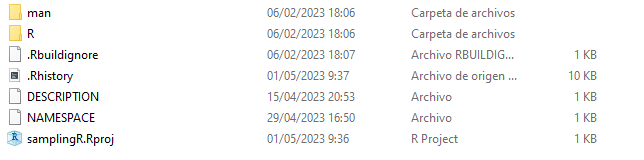
\includegraphics[scale=0.8]{img/proyecto.png}
    \captionof{figure}{Estructura de un proyecto en R.}
    \label{fig:proj}
\end{center}

Los contenidos que figuran dentro de esta carpeta de forma resumida son los siguientes:\\

\begin{itemize}[label=$\bullet$]
    \item man: carpeta donde se encuentran los ficheros de documentación de las funciones.
    \item R: carpeta donde se encuentran los archivos con extensión .R de funciones.
    \item DESCRIPTION: archivo donde se almacena información importante sobre el paquete.
    \item NAMESPACE: archivo donde se encuentran los nombres de funciones públicas al usuario y menciones sobre el uso de otras librerías de funciones en caso de requerir de sus funciones en algún momento del desarrollo.
    \item Archivo .Rproj: archivo que se usa para abrir el proyecto en una nueva sesión R.
\end{itemize}

Dependiendo de los archivos a crear pueden generarse carpetas adicionales, como explicamos en la sección dedicada a la creación de viñetas \ref{sect:3.4}
Una vez obtenida toda esta estructura, ya se podría crear un nuevo archivo de funciones dentro de la carpeta \textit{R} con el código deseado.\\

\section{Documentación de funciones}
Un apartado muy importante y  que constituye buena práctica a la hora de escribir una nueva función es la documentación. En R resulta particularmente útil definirla ya que gracias a la librería \textit{roxygen2} \cite{Roxygen2} la documentación incluida en las funciones será traducida a archivos legibles por el usuario que aparecerán en la sección \textit{Ayuda} al acceder a la documentación de dicha función, lo que facilita al usuario final  comprender mejor cuál es el objetivo de esa función. Para empezar a documentar se debe introducir el carácter \textbf{\#\textquotesingle} y utilizar un indicador adecuado, empezando con \textbf{@}, siendo los más usados los siguientes:
\\
\begin{itemize}[label=$\bullet$]
    \item title: Descripción general de la función. Indica el propósito de la función de forma breve.
    \item description: Ampliación del propósito de la función.
    \item param: Primero indica el nombre del parámetro dentro de la función y seguido de un espacio lo que representa para la función. Debe haber tantos como parámetros tenga la función.
    \item return: Indica si la función devuelve un objeto del tipo de objeto que se trata y sus contenidos si es conveniente.
    \item details: Sirve para ampliar información acerca de la función que no tenga cabida en el apartado de descripción como funcionamiento interno de la función o valores específicos de parámetros.
    \item references: En caso de querer aportar referencias teóricas sobre las que se fundamenta el código realizado.
    \item examples: Permite escribir una caso de uso de la función para referencia del usuario.
    \item importFrom: Indica que se ha hecho uso de una función externa durante el desarrollo de la función. Se utiliza escribiendo el nombre de la librería y el de la función utilizada separadas por espacios.
    \item export: Hace pública la función al usuario.
    
\end{itemize}

En ocasiones, habrá funciones de uso recurrente que se usan para comodidad a la hora de desarrollar las funciones principales, y que no es necesario ponerlas a disposición de usuario final. Es una buena práctica que estas funciones ``auxiliares'' sean documentadas como cualquier otra de nuestra librería.\\

Sin embargo, esta práctica sin más, implica su publicación al usuario general y por lo tanto aparecerán en el manual y serán accesibles por los usuarios finales. Si no queremos que esto ocurra, se deberá eliminar el indicador \textit{@export} y sustituirlo por \textit{@noRd}. De esta forma disponemos de la documentación de la función en el fichero de código, pero no aparecerá en el manual ni en la sección \textit{Ayuda}. Tampoco será accesible por el usuario final, al menos no de la forma convencional, es decir con el nombre de la función o bien con el formato \textit{librería::función}.\\

Es posible acceder a ellas utilizando tres puntos dobles, por ejemplo, \textit{samplingR:::all01list} nos permite utilizar una función auxiliar que se utiliza en este trabajo en el control de funciones para comprobar que todos los valores de todas las entradas de una lista son ceros o unos. Es un caso no deseable pero es la forma más parecida de lograr el equivalente a funciones denominadas ``privadas'' de otros lenguajes de programación.\\

\section{Librería devtools}
Devtools \cite{devtools} es una herramienta que facilita la creación y desarrollo de librerías en R. Proporciona funciones de gran utilidad y que son muy recomendables a la hora de fijar un flujo de trabajo en el desarrollo. Entre ellas podemos destacar las siguientes:\\
\begin{itemize}[label=$\bullet$, font=\bfseries]
    \item document(): traduce los comentarios en formato Roxygen2 \cite{Roxygen2} de tus funciones a archivos .md de ayuda y crea el archivo NAMESPACE actualizado. La primera vez que se ejecuta es conveniente borrar el archivo NAMESPACE creado por defecto para que escriba los nombres de tus funciones.
    
    \item check(): hace un test automatizado similar al que se ejecuta cuando realizas tu petición de subida a CRAN \cite{CRAN}. Informa de errores, avisos y notas en el paquete. También existen funciones más específicas para comprobar concretamente la documentación o si cumple los requisitos para sistemas operativos Mac o Windows. Si se utiliza RStudio también es posible hacerlo en la parte superior derecha de la interfaz, donde suele encontrarse las variables de entorno. Pestaña Build $\Rightarrow$ Check 
    
    \item build(): genera un archivo comprimido con extensión .tar.gz preparado para ser instalado o subido a CRAN \cite{CRAN}. Al igual que con \textit{check()} también existen métodos para generar el manual de uso de la librería o viñetas de las que se hablará más adelante. En la interfaz de RStudio Build $\Rightarrow$ More $\Rightarrow$ Build Source Package.
\end{itemize}

\begin{center}
    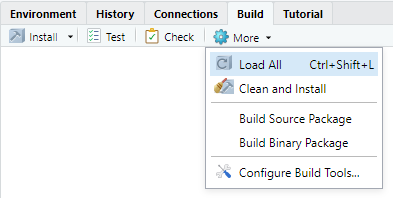
\includegraphics[scale=0.7]{img/build.png}
    \captionof{figure}{Uso de funciones de devtools desde la interfaz gráfica.}
    \label{fig:build}
\end{center}

De forma excepcional y en pocas ocasiones, es posible que al realizar check() se reciba una nota indicando que ha sido imposible comprobar la hora. Es un error que se debe a que la fecha la verifica a través de \textit{Word Clock API} \cite{worldclock} y el servicio está temporalmente inoperativo, por lo que puede ser ignorado o reintentarse más adelante.\\

\section{Creación de viñetas} \label{sect:3.4}
Generalmente, la documentación de las funciones  ayuda a dar una idea general del uso de una función específica, pero no siempre va acompañada de ejemplos de uso o esta ayuda no queda lo suficientemente clara para comprender en detalle el resultado que se pueda obtener con esas funciones. \\

Una solución útil para hacer frente al problema anterior es la creación de viñetas, las cuales se diseñan con la finalidad de mostrar la utilidad de una librería o de parte de sus funciones en su conjunto mediante la resolución de un problema propuesto. Aparecen en la ayuda del paquete antes del listado de funciones y se pueden realizar múltiples viñetas para abarcar los casos de uso más importantes para aquellas librerías de mayor extensión.\\

Para generar una viñeta se puede usar el comando \textit{usethis::use\_vignette("nombre")}. Si se trata de la primera, se creará una carpeta en la raíz del directorio del paquete con nombre \textit{vignettes}, donde se almacenarán las viñetas creadas junto a un archivo \textit{.gitignore} para evitar que los archivos creados pasen control de versiones, además de añadir las dependencias al archivo \textit{DESCRIPTION}. Dentro de la carpeta aparecerá un archivo .Rmd (es decir, se trataría de un archivo de tipo Rmarkdown) con el nombre de nuestra viñeta. En él encontramos dos bloques de código: el primero destinado a incluir los metadatos de la viñeta, como su título y forma de presentación, que puede ser como un archivo HTML, PDF, un cuaderno de trabajo similar a los cuadernos Jupiter de Python, etc. El segundo bloque incluye los ajustes predeterminados de presentación del código y sus resultados. El último simplemente realiza la llamada de nuestra librería para poder empezar a trabajar.\\


\section{Petición de subida a CRAN}
En el supuesto de que se decida subir la librería al repositorio oficial para uso general de todos los usuarios, se deberá ir al sitio web dedicado a la realización de esta acción, accesible desde la página oficial. Previamente se deberá realizar algunas modificaciones a los contenidos del paquete para poder enviarlo.\\

El archivo DESCRIPTION contiene la información principal de la librería, tal como su nombre o las personas que lo han desarrollado. Debe ser rellenado con la información pertinente. Entre sus campos encontramos: \\

\begin{itemize}[label=$\bullet$]
    \item \textit{Package}, que especifica el nombre de la librería. Éste no puede coincidir con el de ningún otro subido a CRAN con anterioridad. Los nombres son case-insensitive, por lo que, por ejemplo, samplingr no será aceptado por coincidir con el nombre de la librería de este trabajo. La forma más cómoda de buscar un nombre es ir a \textit{install} de la pestaña \textit{Packages} de RStudio  y escribir el nombre elegido, ya que con el autocompletado podrás ver los nombres con coincidencia parcial al texto introducido.
    \item \textit{Title} muestra el título que aparecerá en la página general de ayuda del paquete. Se trata de una única frase escrita en title-case, por lo que exceptuando artículos, preposiciones y similar la primera letra de las palabras debe ser mayúscula. No debe terminar en punto, ya que de lo contrario se nos avisará al subirlo al repositorio de CRAN. Tampoco conviene poner ``en R'' ya que los revisores lo consideran error por reiterativo. 
    \item \textit{Maintainer} indica la persona que lleva a cabo tareas de mantenimiento de la librería. Es importante que la información sea correcta ya que se usará para comunicar novedades sobre el estado del paquete durante el proceso de revisión y subida. Sigue el formato nombre apellido $<$correo electrónico$>$ 
    \item \textit{Authors@R} indica las personas involucradas en el desarrollo del paquete. Anteriormente se usaba un formato similar al de Maintainer, pero ahora se aconseja usar la clase \textit{person} \cite{person}. Dispone de múltiples roles para asignar a cada persona en función del trabajo realizado. 
    \item \textit{Description} amplía la información del título sobre el uso de la librería. Hay que ser moderadamente específicos con lo que realiza ya que si usas términos como \textit{diferentes funciones o varios métodos} los revisores pueden exigir elaborar sobre dichos métodos.
    \item \textit{Version} indica la versión de desarrollo de la librería. Por defecto se sitúa en 0.1.0. Es importante que cada vez que subamos una actualización del paquete al repositorio modifiquemos manualmente este valor ya que de lo contrario se detectará una coincidencia y la subida no será efectiva.
\end{itemize}

Una vez tengamos el archivo \textit{DESCRIPTION} completo, rellenaremos el formulario haciendo que el nombre y correo electrónico coincidan con los del \textit{Maintainer} y subiremos un archivo con extensión .tar.gz creado previamente con la función build(). Pasados unos minutos después del envío, llegará al correo del maintainer un mensaje de confirmación con un enlace donde se deben aceptar los términos.\\

Si nos fijamos en el segundo de estos términos, confirmamos haber realizado una comprobación de tipo check() y nos adjunta una página web. Esto se debe a que según las directrices de CRAN es necesario realizar comprobaciones como las de la función check(), pero siguiendo las normas de la próxima versión de R planeada para ser desplegada.\\

Existen dos formas de realizar estas comprobaciones. La primera es instalar R-devel, es decir la siguiente versión de R en tu ordenador para realizar ahí las comprobaciones. Este método puede resultar pesado, por lo que si entramos al enlace mencionado anteriormente veremos un lugar donde realizar comprobaciones para la versión actual, anteriores o R-devel. Solo hace falta subir el archivo con extensión .tar.gz e indicar el correo donde se quiera recibir el resultado y en cuestión de minutos llegará un enlace a un archivo tipo log donde veremos los resultados de la misma manera que realizando check() en local. En el mejor caso recibiremos solo una nota encima del maintainer, lo cual es normal ya que se trata de un recordatorio para que los maintainer comprueben en los ficheros log que la actualización ha sido solicitada por él y no otra persona, según Uwe Ligges, maintainer de CRAN.\\


\begin{figure}[H]
    \centering
    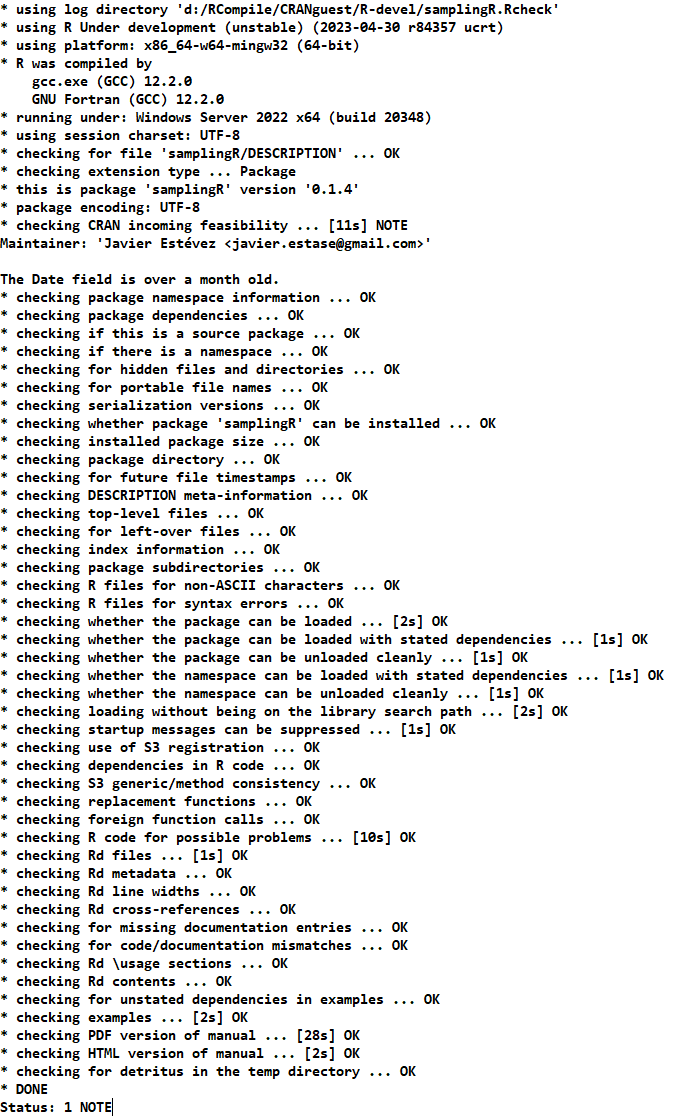
\includegraphics[scale=0.4]{./img/winbuilder.png}
    \caption{Ejemplo de resultados usando la herramienta Winbuilder.}
    \label{fig:enter-label}
\end{figure}

Una vez confirmados los términos llegará un segundo correo con los resultados de los tests automatizados. En cualquier caso, se notificará del resultado y se tendrá acceso al registro completo en un archivo tipo log. Una confusión generalizada al ver este archivo es ver una nota en el nombre del maintainer. En caso de pasar los tests se añadirá que el paquete queda pendiente de una última revisión manual. Esta última revisión será la que más se demore en la entrega de  sus resultados y es aquí donde pueden sugerir cambios que no muestre la función check() como los antes mencionados del archivo DESCRIPTION, usar TRUE y FALSE en lugar de sus homónimos T y F en el código para mejorar su comprensión o reformular descripciones de funciones que contienen ``esta función...'' por redundantes.\\

Tras recibir el visto bueno por parte de los moderadores, su respuesta será una confirmación de que el paquete se ha creado correctamente y se encuentra de camino a CRAN. Generalmente se estima un periodo de 24 horas antes de poder ser descargado por los usuarios.\\




\newpage
\chapter{Muestreo aleatorio simple}

El muestreo aleatorio simple es una de las técnicas más sencillas de tomar una muestra de una población, ya que se basa en la selección de unidades de forma individual y aleatoriamente, según un modelo uniforme discreto, por lo que todos los individuos de la población tienen la misma probabilidad de ser elegidos.\\

En la práctica, para seleccionar las muestras mediante este tipo de muestreo se requiere la existencia de un marco que identifique las unidades de muestreo, que son precisamente los elementos de la población. En España, para las estadísticas oficiales dirigidas a la población, este marco de muestreo se basa principalmente en los datos obtenidos del padrón municipal de habitantes, del cual se pueden extraer tanto individuos como hogares facilitando de esta manera una información sumamente valiosa de cara a diseñar diferentes tipos de muestreo. Para el caso de muestras dirigidas a empresas, el INE utiliza el Directorio Central de Empresas (DIRCE) \cite{DIRCE}, el cual reúne en un sistema de información único a todas las empresas española y a sus unidades locales ubicadas en el territorio nacional. Su objetivo básico es hacer posible la realización de encuestas económicas por muestreo. \\

Existen dos variantes de este tipo de muestreo según las características de sus muestras. El muestreo sin reposición impide la posibilidad de incluir individuos repetidos en la muestra a diferencia del muestreo con reposición, lo que repercute en la estimación de parámetros.\\

Tanto en el muestreo sin reemplazamiento como con reemplazamiento la probabilidad de inclusión en la muestra para todos los individuos de la población es:\\
\begin{equation}\label{eq:1}
    \pi_i = \frac{n}{N}
\end{equation}

donde n es el tamaño de la muestra deseada y N el tamaño poblacional.

\section{Selección de muestras} \label{sect:3.1}
La selección de la muestra sobre la que estudiar la variable de interés debe seguir un procedimiento que asegure la aleatoriedad del proceso. Generalmente se distinguen dos procedimientos con sus posibles aplicaciones en el campo de la informática.\\

El método de la urna se basa en introducir todos los elementos de la población en una urna, convenientemente removida, para sacar uno a uno elementos hasta llegar al tamaño de muestra deseado. Al no poder ver el interior de la urna se supone aleatoriedad.\\

En el muestreo con reposición, tras seleccionar un individuo, éste debe ser devuelto a la urna para permitir que pueda salir elegido de nuevo. En el caso de muestreo sin reposición, cada elemento seleccionado no se devuelve a la urna\\

Para lograr un método de selección similar en un programa informático, se deben enumerar las unidades poblacionales del 1 a N, siendo N el tamaño poblacional. Después utilizando un método aleatorio se obtiene un número aleatorio entre 1 y N, obteniendo el índice del individuo seleccionado. El procedimiento se repite tantas veces como muestras se requieran. En el muestreo sin reposición tras la selección de cada individuo éste se retiraría de la lista y sería necesario tener un control extra sobre el número aleatorio para que no se repita. Un ejemplo sería seleccionar uno nuevo si coincide con el índice de algún individuo seleccionado previamente.\\

El segundo método consiste en usar tablas de números aleatorios, donde se crea una secuencia de números entre 1 y N. Se elige un punto de partida y se seleccionan tantos elementos de forma secuencial como requiera la muestra. Para ello es preciso numerar los individuos al igual que en el método anterior.\\

\begin{center}
    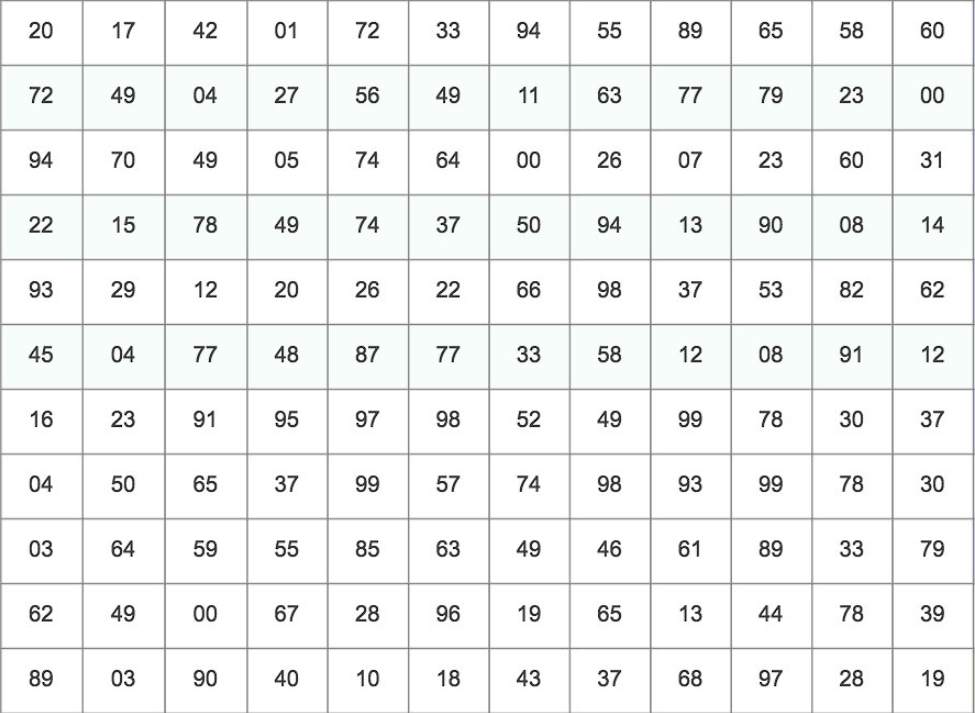
\includegraphics[scale=0.4]{img/tablanumeros.png}
    \captionof{figure}{Ejemplo de tabla de números aleatorios.}
    \label{fig:tablanumeros}
\end{center}

Tomando como ejemplo la figura \ref{fig:tablanumeros} para la selección de una muestra en una población de tamaño 100, se parte desde el primer número, y se seleccionan los números necesarios en orden, bien siguiendo las filas o las columnas, ya que no afecta a la aleatoriedad de la selección. En el caso de querer una muestra de tamaño 5 tomaremos los 5 primeros números de izquierda a derecha o de  arriba hacia abajo, por lo que nuestra muestra constará de los individuos de la población numerados con los índices 20, 17, 42, 1 y 72.\\

Para su aplicación en software informático se indexan los individuos y se utiliza un generador aleatorio de números para obtener tantos números entre 0 y 1 como individuos existen en la población. De entre esos números se seleccionan tantos valores como se requieran para la muestra siguiendo una regla como por ejemplo, utilizando los valores más grandes o los más pequeños, etc. Haciendo coincidir el índice de dichos números con la numeración de la población obtenemos los individuos que forman la muestra aleatoria.\\

En éste trabajo se ha utilizado el método de la urna para la selección de muestras con reemplazamiento y las tablas de números aleatorios para el caso sin reemplazamiento.\\


\section{Estimadores lineales insesgados} \label{sect:3.2}
\subsection{Muestreo aleatorio simple sin reemplazamiento}
Tomando el estimador de Horwitz-Thompson como el estimador lineal insesgado general podemos obtener los estimadores lineales insesgados de los parámetros que precisamos. En concreto, tenemos:\\
\begin{equation}\label{eq:2}
    \hat{\theta}_{HT} = \sum_{i=1}^{n}\frac{Y_i}{\pi_i}
\end{equation}

Para obtener el estimador del total poblacional realizamos el siguiente desarrollo:\\

\begin{equation}\label{eq:3}
    \theta = X = \sum_{i=1}^{N}X_i \Rightarrow Y_i = Xi \Rightarrow \hat{\theta} = \hat{X} = \sum_{i=1}^{n}\frac{X_i}{\pi_i} = \sum_{i=1}^{n}\frac{X_i}{\frac{n}{N}} = N\frac{1}{n}\sum_{i=1}^{n}X_i = N\bar{x}
\end{equation}

Sustituyendo de forma similar para los parámetros media, proporción y total de clase tenemos:\\
\begin{equation}\label{eq:4}
    \hat{\theta} = \hat{\bar{X}} = \sum_{i=1}^{n}\frac{\frac{X_i}{N}}{\pi_i} = \sum_{i=1}^{n}\frac{\frac{X_i}{N}}{\frac{n}{N}} = \frac{1}{n}\sum_{i=1}^{n}X_i = \bar{x}
\end{equation}

\begin{equation}\label{eq:5}
    \hat{\theta} = \hat{P} = \sum_{i=1}^{n}\frac{A_i}{\pi_i} = \sum_{i=1}^{n}\frac{\frac{A_i}{N}}{\frac{n}{N}} = \frac{1}{n}\sum_{i=1}^{n}A_i = P
\end{equation}

\begin{equation}\label{eq:6}
    \hat{\theta} = \hat{A} = \sum_{i=1}^{n}\frac{A_i}{\pi_i} = \sum_{i=1}^{n}\frac{A_i}{\frac{n}{N}} = N\frac{1}{n}\sum_{i=1}^{n}A_i = NP
\end{equation}
Donde $A_i$ son observaciones de una variable dicotómica con valores 0 ó 1.\\

\subsection{Muestreo aleatorio simple con reemplazamiento}
Como ya comentamos al principio de la sección, la probabilidad de inclusión en la muestra para este tipo de muestreo es igual que para el muestreo sin reemplazamiento, por lo que sus estimadores lineales insesgados serán equivalentes a los de las fórmulas \ref{eq:3} a \ref{eq:6}.\\


\section{Estimadores de la varianza} \label{sect:3.3}
\subsection{Muestreo aleatorio simple sin reemplazamiento}

Partiendo de la expresión general del estimador insesgado para el cálculo de la varianza en el muestreo sin reposición:\\

\begin{equation}\label{eq:7}
    \widehat{V(\hat{\theta}_{HH})} = \sum_{i=1}^{n}\frac{Y_i^2}{\pi_i^2}(1-\pi_i) +  \sum_{i<j}^{n}\frac{Y_iY_j}{\pi_i\pi_j}\frac{\pi_{ij}-\pi_i\pi_j}{\pi_{ij}}
\end{equation}

y sustituyendo para los estimadores tenemos: \\

\begin{equation}\label{eq:8}
    \hat{V}(\hat{X}) = N^2(1-f)\frac{\hat{S}^2}{n}
\end{equation}
\begin{equation}\label{eq:9}
    \hat{V}(\hat{\bar{X}}) = (1-f)\frac{\hat{S}^2}{n}
\end{equation}    
\begin{equation}\label{eq:10}
    \hat{V}(\hat{P}) = (1-f)\frac{\hat{P}\hat{Q}}{n-1}
\end{equation}
\begin{equation}\label{eq:11}
    \hat{V}(\hat{A}) = N^2(1-f)\frac{\hat{P}\hat{Q}}{n-1}
\end{equation}

donde $f=\frac{n}{N}$ y la cuasivarianza muestral es un estimador insesgado de la cuasivarianza poblacional, y queda definida por:\\

\begin{equation}\label{eq:12}
    \hat{S}^2 = \frac{1}{n-1}\sum_{i=1}^{n}(X_i-\bar{x})^2
\end{equation}

\subsection{Muestreo aleatorio simple con reemplazamiento} \label{sect:4.3.2}
La expresión general del estimador insesgado de la varianza en el muestreo aleatorio con reemplazamiento es:\\
\begin{equation}\label{eq:13}
    \widehat{V(\hat{\theta}_{HH})} = \frac{1}{n-1}\sum_{i=1}^{n}(\frac{Y_i}{P_i}-\hat{Y}_{HH})^2
\end{equation}

que al aplicarla al estimador del total, media, proporción y total de clase obtenemos:\\

\begin{equation}\label{eq:14}
    \hat{V}(\hat{X}) = N^2\frac{\hat{S}^2}{n}
\end{equation}
\begin{equation}\label{eq:15}
    \hat{V}(\hat{\bar{X}}) = \frac{\hat{S}^2}{n}
\end{equation}    
\begin{equation}\label{eq:16}
    \hat{V}(\hat{P}) = \frac{\hat{P}\hat{Q}}{n-1}
\end{equation}
\begin{equation}\label{eq:17}
    \hat{V}(\hat{A}) = N^2\frac{\hat{P}\hat{Q}}{n-1}
\end{equation}

donde la cuasivarianza muestral $\hat{S}^2$ es un estimador insesgado de la varianza poblacional.\\

Como puede comprobarse estas expresiones son equivalentes a las expresiones \ref{eq:8} a \ref{eq:11} del muestreo sin reposición excepto el factor $(1-f)$.\\
    

\section{Tamaño de la muestra} \label{sect:3.4}
Cuando se realiza el estudio de una variable de interés sobre una población mediante técnicas de muestreo, es deseable que al realizar la estimación se aseguren unas tolerancias en el error.\\

Desarrollando la expresión del error de muestreo e = $\sqrt{ \hat{V}(\hat{\theta})}$ y despejando n se puede obtener el tamaño de muestra que debería tomarse dependiendo del estimador y el tipo de muestreo realizado para lograr los resultados deseados.\\

Las diferentes situaciones que se han usado en este trabajo, son las siguientes:\\

\subsection{Error de muestreo dado}\label{sect:4.4.1}
Es el escenario más simple, en el que determinamos el tamaño de la muestra en base al error de muestreo absoluto a cometer. Tomamos el ejemplo de la estimación para la media en el muestreo aleatorio sin reemplazamiento:\\
\begin{equation}
    e = \sqrt{ \hat{V}(\hat{\theta})} = \sqrt{(1-\frac{n}{N})\frac{S^2}{n}} \Rightarrow n = \frac{NS^2}{Ne^2+S^2} 
\end{equation}

Al tomar muestras con este tamaño es posible que el error de muestreo sea ligeramente mayor que el especificado, pero siempre será cercano a su valor.\\

\subsection{Error de muestreo y coeficiente de confianza dados}\label{sect:4.4.2}
En el caso en el que se desea obtener un error de muestreo menor o igual al especificado de forma más consistente que en el anterior escenario es necesario introducir un coeficiente de confianza $\alpha$ entre 0 y 1 de forma que con probabilidad $1-\alpha$ nos encontremos en la situación deseada.\\

Para ello tomamos $\lambda_\alpha$ como el cuartil de la distribución normal estándar para el valor de $\alpha$ dado. Desarrollando la expresión de la media:\\
\begin{equation}
    e_\alpha = \lambda_\alpha e= \sqrt{(1-\frac{n}{N})\frac{S^2}{n}} \Rightarrow n = \frac{\frac{\lambda_\alpha^2S^2}{e_\alpha^2}}{1+\frac{\frac{\lambda_\alpha^2S^2}{e_\alpha^2}}{N}} = \frac{n_\alpha}{1+\frac{n_\alpha}{N}} 
\end{equation}
Al introducir el coeficiente de confianza el valor de n siempre será mayor que en el apartado \ref{sect:4.4.1}\\

\subsection{Error relativo de muestreo dado}\label{sect:4.4.3}
El error relativo representa otra medida de precisión distinta al error de muestreo y se define como el coeficiente del error de muestreo sobre el parámetro y el valor del parámetro sobre la población, o lo que es lo mismo su valor real.\\
\begin{equation}
    e_r = \frac{ \sqrt{\widehat{V(\bar{X})}} }{E(\bar{X})} = \frac{\sqrt{(1-\frac{n}{N})\frac{S^2}{n}}}{\bar{X}} \Rightarrow n = \frac{N(\frac{S}{\bar{X}})^2}{e_r^2+\frac{(\frac{S}{\bar{X}})^2}{N}} = \frac{NC^2}{e_r^2+\frac{C^2}{N}}
\end{equation}
    
\subsection{Error relativo de muestreo y coeficiente de confianza dados}
Siguiendo la propuesta del apartado \ref{sect:4.4.2} y la expresión del error relativo del apartado \ref{sect:4.4.3} tenemos: \\
\begin{equation}
    e_{r\alpha} = \lambda_\alpha \frac{ \sqrt{\hat{V}(\bar{X})} }{E(\bar{X})} \Rightarrow n = \frac{\lambda_\alpha^2 C^2}{e_{r\alpha}^2 + \lambda_\alpha^2\frac{C^2}{N}}
\end{equation}

Desarrollando para el resto de parámetros y en ambos tipos de muestreo finalmente tenemos:\\
\subsection{Muestreo aleatorio simple sin reemplazamiento}

Se incluye en este apartado un resumen de las fórmulas para estimar los tamaños de muestra en el muestreo irrestricto aleatorio, agrupadas en la tabla \ref{tab:srssamplesize}.\\


\begin{table}[H]
\centering
\begin{tabular}{|c|c|c|c|c|}
\hline
\begin{tabular}[c]{@{}c@{}}Tipo de error\\ Parametro\end{tabular} & Absoluto & Relativo & \begin{tabular}[c]{@{}c@{}}Absoluto y coeficiente \\ de confianza adicional\end{tabular} & \begin{tabular}[c]{@{}c@{}}Relativo y coeficiente\\  de confianza adicional\end{tabular} \\ \hline
Total   &  $\frac{N^2 S^2}{e^2+N S^2}$        &  $\frac{N C^2}{N e_r^2+C^2}$        &  $\frac{\lambda_\alpha^2 N^2 S^2}{e^2+\lambda_\alpha^2 N S^2}$   &            $\frac{\lambda_\alpha^2 N C^2}{N e_{r \alpha}^2+\lambda_\alpha^2 C^2}$               \\ \hline
Media   &   $\frac{N S^2}{N e^2+S^2}$       &    $\frac{N C^2}{N e_r^2+C^2}$      &     $\frac{\lambda_\alpha^2 N S^2}{N e^2+\lambda_\alpha^2 S^2}$    &     $\frac{\lambda_\alpha^2 N C^2}{N e_{r \alpha}^2+\lambda_\alpha^2 C^2}$   \\ \hline
Proporción   &  $\frac{N P Q}{e^2(N-1)+P Q}$        &   $\frac{N Q}{P(N-1) e_r^2+Q}$       &     $\frac{\lambda_\alpha^2 N P Q}{e^2(N-1)+\lambda_\alpha^2 P Q}$  &   $\frac{N Q \lambda_\alpha^2}{e_{r \alpha}^2(N-1) P+\lambda_\alpha^2 Q}$                      \\ \hline
Total de clase  &     $\frac{N^3 P Q}{e^2(N-1)+N^2 P Q}$ &   $\frac{N Q}{P(N-1) e_r^2+Q}$     &         $\frac{\lambda_\alpha^2 N^3 P Q}{e^2(N-1)+\lambda_\alpha^2 N{ }^2 P Q} $ & $\frac{N Q \lambda_\alpha^2}{e_{r \alpha}^2(N-1) P+\lambda_\alpha^2 Q}$  \\ \hline
\end{tabular}
\caption{Tamaños de muestra en el muestreo aleatorio simple sin reemplazamiento.}
\label{tab:srssamplesize}
\end{table}

\subsection{Muestreo aleatorio simple con reemplazamiento}

En la tabla \ref{tab:srssamplesize2} se resumen las fórmulas de estimación del tamaño poblacional en el caso del muestreo aleatorio simple con reemplazamiento.\\


\begin{table}[H]
\centering
\begin{tabular}{|c|c|c|c|c|}
\hline
\begin{tabular}[c]{@{}c@{}}Tipo de error\\ Parametro\end{tabular} & Absoluto & Relativo & \begin{tabular}[c]{@{}c@{}}Absoluto y coeficiente \\ de confianza adicional\end{tabular} & \begin{tabular}[c]{@{}c@{}}Relativo y coeficiente\\  de confianza adicional\end{tabular} \\ \hline
Total  &  $\frac{N^2 \sigma^2}{e^2}$    &  $\frac{C^2}{e_r^2}$  &   $\frac{\lambda_\alpha^2 N^2 \sigma^2}{e^2}$   & $\frac{\lambda_\alpha^2 C^2}{e_{r \alpha}^2}$  \\ \hline
Media      &   $\frac{\sigma^2}{e^2}$    &   $\frac{C^2}{e_r^2}$   &    $\frac{\lambda_\alpha^2 \sigma^2}{e^2}$    & $\frac{\lambda_\alpha^2 C^2}{e_{r \alpha}^2}$     \\ \hline
Proporción     &   $\frac{P Q}{e^2}$       &   $\frac{Q}{P e_r^2}$       &   $\frac{\lambda_\alpha^2 P Q}{e^2}$        &     $\frac{\lambda_\alpha^2 Q}{P e_{r \alpha}^2}$                 \\ \hline
Total de clase        &   $\frac{N^2 P Q}{e^2}$       &   $\frac{Q}{P e_r^2}$       &     $\frac{N^2 \lambda_\alpha^2 P Q}{e^2}$            &          $\frac{\lambda_\alpha^2 Q}{P e_{r \alpha}^2}$            \\ \hline
\end{tabular}
\caption{Tamaños de muestra en el muestreo aleatorio simple con reemplazamiento.}
\label{tab:srssamplesize2}
\end{table}


\section{Dominios de estudio} \label{sect:3.5}
Es posible que dentro de la población los individuos estén divididos en subpoblaciones o dominios de los cuales interesa estudiar la variable de interés sobre una de ellas. El problema reside en que no siempre el marco de estudio permite muestrear la subpoblación deseada hasta que no se evalúan los individuos de un marco más general. \\

Una vez tomada una muestra y etiquetados sus individuos en dominios, es posible estudiar la variable de interés para dicho dominio. Para el caso de la media de un dominio tendríamos:
\begin{equation}
    \hat{\bar{Y_j}} = \sum_{k=1}^{n_j}Y_{jk}
\end{equation}
Donde $Y_{jk}, k=1...n_j$ son las medidas de la variable de interés para cada individuo del dominio y $n_j$ el tamaño del dominio dentro de la muestra.\\

Para la estimación de la varianza usaríamos 
\begin{equation}
    \widehat{V(\hat{\bar{Y_j}})} = (1-\frac{n_j}{N_j})\frac{\hat{S_j^2}}{n_j}
\end{equation}
Donde $\hat{S_j^2}$ es la cuasivarianza muestral del dominio y $N_j$ el tamaño del dominio en la población. En caso de no conocer éste último parámetro se puede realizar la aproximación $\frac{n_j}{N_j} = \frac{n}{N}$. \\

\section{Aplicaciones en la librería samplingR}

Las funciones desarrolladas para la aplicación de los conceptos teóricos mostrados anteriormente utilizarán el prefijo \textit{srs} como abreviación de \textit{simple random sampling}, y son las siguientes.

\begin{itemize}[label=$\bullet$]
    \item srs.sample: Dado un tamaño poblacional N y un tamaño de muestra n devuelve una muestra aleatoria simple. Dicha muestra puede ser tomada con o sin reemplazamiento, dependiendo del valor del parámetro \textit{replace}. En caso de aportar un conjunto de datos devolverá los individuos de los datos que conforman la muestra. Al ser esto opcional, si no se aporta un conjunto de datos devolverá los índices de los individuos que conforman la muestra.\\

    Realiza las funciones explicadas en el apartado \ref{sect:3.1}.

    \item srs.estimator: Dada una muestra de datos obtiene el estimador poblacional del parámetro especificado, entre \textit{total poblacional}, \textit{media}, \textit{proporción} y \textit{total de clase}. También calcula su varianza estimada, error de muestreo y opcionalmente su error de estimación y un intervalo de confianza si se especifica el coeficiente de confianza en el parámetro \textit{alpha}. \\

    Se permite especificar si el muestreo se realiza con o sin reemplazamiento para realizar estimaciones más precisas.\\

    Realiza las funciones explicadas en el apartado \ref{sect:3.2} y \ref{sect:3.3}.

    \item srs.domainestimator: Realiza las mismas estimaciones de la función anterior, pero sobre una subpoblación o dominio de los datos muestrales.\\

    Realiza las funciones explicadas en el apartado \ref{sect:3.5}.

    \item srs.samplesize: Calcula el tamaño de muestra necesario para cometer un error de muestreo menor del especificado. Dicho error puede ser absoluto o relativo, según el parámetro \textit{relative}, y se permite la relajación de su estimación si se especifica un coeficiente de confianza. \\

    Para la estimación no se pide aportar los datos poblacionales por la posibilidad de no disponer de ellos, si no que se deben aportar medidas estadísticas tales como la estimación de la varianza y el tamaño poblacional. También se puede especificar el tipo de muestreo que se va a utilizar para realizar estimaciones más precisas.\\

    Aplica los conceptos explicados en el apartado \ref{sect:3.4}.


\end{itemize}



\newpage
\chapter{Muestreo estratificado}
El objetivo del muestreo estratificado consiste en dividir una población heterogénea en subpoblaciones no solapadas lo más homogéneas posibles llamadas estratos, los cuales pueden venir determinados por factores demográficos, geográficos, socioeconómicos u otras variables relevantes para el estudio.\\

Gracias a esta estrategia es posible representar de manera más precisa la información de los distintos estratos, teniendo en cuenta la heterogeneidad que hay  entre ellos. Además podemos realizar inferencias sobre cada uno de los estratos estudiados. Otra ventaja de esta división es la de poder destinar más recursos en la recogida de una muestra en aquellos estratos con mayor variabilidad para así ganar precisión reduciendo el error de muestreo.\\

Este tipo de muestreo es un método poderoso y flexible que es ampliamente usado en la práctica. En las encuestas económicas (son las dirigidas a las empresas) es el principal tipo de diseño utilizado. Por ejemplo, se utiliza por el INE en los cálculos del \textit{Índice de Comercio al por Menor} o la \textit{Estadística Estructural de Empresas}.\\

\section{Selección de la muestra} \label{sect:4.1}
Para formar una muestra estratificada basta con tomar una muestra aleatoria (existen métodos para utilizar diferentes tipos de muestreo que además no debe de ser el mismo en cada estrato) para cada uno de los estratos en los que se divide la población. De este procedimiento surge una nueva cuestión: ¿Cómo realizamos el reparto del tamaño muestral entre los diferentes estratos?\\

La \textit{afijación} de la muestra es el nombre con el que se denomina esta adjudicación de tamaños de submuestra para cada uno de los estratos. Entre las más destacadas y utilizadas en la práctica, se encuentran la afijación uniforme, proporcional, de mínima varianza y óptima, que vemos a continuación.\\

\subsection{Afijación uniforme} \label{sect:4.1.1}
Se trata de la estrategia más sencilla, consistente en asignar el mismo número de individuos a la muestra de cada uno de los estratos, teniendo entonces que $n_h = \frac{n}{L}$ $\forall h=1,...,L$ donde L es el número de estratos. En el caso de que $\frac{n}{L}$ no sea un número entero $n_h$ se redondea según sea conveniente para que al final nos acerquemos lo máximo posible al tamaño muestral deseado.\\
 
\subsection{Afijación proporcional} \label{sect:4.1.2}
Consiste en asignar individuos de la muestra de forma proporcional al tamaño poblacional de cada estrato, asegurando así la equiprobabilidad de que un individuo de la población pertenezca a la muestra, con una probabilidad de inclusión de $\pi_{hi} = \frac{n_h}{N_h}$. \\

Con este tipo de afijación, el tamaño de la muestra para cada estrato queda definido por:
\begin{equation}
    n_h = N_h\frac{n}{N}
\end{equation}


\subsection{Afijación de mínima varianza} \label{sect:4.1.3}
También conocida como afijación de Neyman, pretende calcular los tamaños de muestra para cada estrato de forma que la varianza de los estimadores sea mínima. Se trata por lo tanto de resolver un problema de optimización en el que queremos minimizar la función objetivo $V(\theta)$ bajo la restricción $\sum\limits_{h=1}^L n_h = n$.\\

El resultado de este problema da la siguiente expresión para el tamaño muestral del estrato h:
\begin{equation}
    n_h = n\frac{N_hS_h}{\sum\limits_{h=1}^LN_hS_h}
\end{equation}

Que coincide para el cálculo del estimador del total y de la media.

\subsection{Afijación óptima} \label{sect:4.1.4}
Este tipo de afijación busca obtener la mínima varianza posible de los estimadores para un coste  fijado C. Este coste será el resultado de la suma de los costes de entrevistar individuos de los diferentes estratos para la muestra, cada uno con un coste determinado. \\

Esto conlleva un problema de optimización con la misma función objetivo que la afijación de Neyman y la restricción $\sum\limits_{h=1}^L c_hn_h = C$, donde $c_h$ representa el coste de entrevistar un individuo del estrato h para la muestra.

Resolviendo el problema llegamos a la expresión:
\begin{equation}
    n_h = n\frac{\frac{N_hS_h}{\sqrt{c_h}}}{\sum\limits_{h=1}^L\frac{N_hS_h}{\sqrt{c_h}}}
\end{equation}

que también coincide para todos los estimadores.\\

Una variante de este enfoque implica añadir al problema anterior un coste máximo de estudio C y opcionalmente un coste base $C_{ini}$, llegando a una expresión similar dada por:

\begin{equation}
    n_h = (C-C_{ini})\frac{\frac{N_hS_h}{\sqrt{c_h}}}{\sum\limits_{h=1}^LN_hS_h\sqrt{c_h}}
\end{equation}

\section{Estimadores lineales insesgados} \label{sect:4.2}
El cálculo de los estimadores lineales en el muestreo estratificado requiere de realizar la suma de los estimadores de todos los estratos, por lo que a partir de la fórmula general del estimador Horwitz-Thompson \ref{eq:2} llegamos a:

\begin{equation}
    \hat{\theta}_{HH} = \sum_{h=1}^{L}\sum_{i=1}^{n_h}\frac{X_{hi}}{\pi_{hi}}
\end{equation}

Extendiendo este procedimiento a las fórmulas \ref{eq:3} a \ref{eq:6} del muestreo aleatorio simple obtenemos:

\begin{equation}
    \hat{\theta} = \hat{X} = \sum_{h=1}^{L}\sum_{i=1}^{n_h}\frac{X_{hi}}{\pi_{hi}} = \sum_{h=1}^{L}\sum_{i=1}^{n_h}\frac{X_{i}}{\frac{n_h}{N_h}} = \sum_{h=1}^{L}N_h\frac{1}{n_h}\sum_{i=1}^{n_h}X_{hi} = \sum_{h=1}^{L}N_h\bar{x_h}
\end{equation}

\begin{equation}
    \hat{\theta} = \hat{\bar{X}} = \sum_{h=1}^{L}\sum_{i=1}^{n_h}\frac{\frac{X_{hi}}{N_h}}{\pi_{hi}} = \sum_{h=1}^{L}\frac{1}{N}\sum_{i=1}^{n_h}\frac{X_{hi}}{\frac{n_h}{N_h}} = \sum_{h=1}^{L}\frac{N_h}{N}\frac{1}{n_h}\sum_{i=1}^{n_h}X_{hi} = \sum_{h=1}^{L}W_h\bar{x_h}
\end{equation}

\begin{equation}
    \hat{\theta} = \hat{P} = \sum_{h=1}^{L}\frac{1}{N}\sum_{i=1}^{n_h}\frac{A_{hi}}{\pi_{hi}} = \sum_{h=1}^{L}\frac{1}{N}\sum_{i=1}^{n_h}\frac{A_{hi}}{\frac{n_h}{N_h}} = \sum_{h=1}^{L}\frac{N_h}{N}\frac{1}{n_h}\sum_{i=1}^{n_h}A_{hi} = \sum_{h=1}^{L}W_hP_h
\end{equation}

\begin{equation}
    \hat{\theta} = \hat{A} = \sum_{h=1}^{L}\sum_{i=1}^{n_h}\frac{A_{hi}}{\pi_{hi}} = \sum_{h=1}^{L}\sum_{i=1}^{n_h}\frac{A_{hi}}{\frac{n_h}{N_h}} = \sum_{h=1}^{L}N_h\frac{1}{n_h}\sum_{i=1}^{n_h}A_{hi} = \sum_{h=1}^{L}N_hP_h
\end{equation}

los cuales coinciden con los estimadores del muestreo estratificado sin reemplazamiento.\\

\section{Estimación de varianzas} \label{sect:4.3}

La estimación de la varianza en cualquier proceso de investigación por muestreo es de suma importancia, ya que gracias a este valor podremos estimar la calidad del estudio realizado. A continuación se procede a relatar cómo se obtiene este valor distinguiendo si el método muestral utilizado es con o sin reemplazamiento.\\

\subsection{Muestreo sin reemplazamiento}
La estimación de la varianza para el estimador $\theta$ es igual a la suma de las varianzas de $\theta$ en cada uno de los estratos al ser las muestras independientes. Sustituyendo $\theta$ por cada uno de los estimadores obtenemos:

\begin{equation}
    \hat{V}(\hat{X}) = \sum_{h=1}^{L}N_h^2(1-f_h)\frac{\hat{S_h}^2}{n_h}
\end{equation}
\begin{equation}
    \hat{V}(\hat{\bar{X}}) = \sum_{h=1}^{L}W_h^2(1-f_h)\frac{\hat{S_h}^2}{n_h}
\end{equation}    
\begin{equation}
    \hat{V}(\hat{P}) = \sum_{h=1}^{L}W_h^2(1-f_h)\frac{\hat{P_h}\hat{Q_h}}{n_h-1}
\end{equation}
\begin{equation}
    \hat{V}(\hat{A}) = \sum_{h=1}^{L}N_h^2(1-f_h)\frac{\hat{P_h}\hat{Q_h}}{n_h-1}
\end{equation}

\subsection{Muestreo con reemplazamiento}
Aplicando el mismo fundamento con las varianzas en el muestreo estratificado con reemplazamiento obtenemos:

\begin{equation}
    \hat{V}(\hat{X}) = \sum_{h=1}^{L}N_h^2\frac{\hat{S_h}^2}{n_h}
\end{equation}
\begin{equation}
    \hat{V}(\hat{\bar{X}}) = \sum_{h=1}^{L}W_h^2\frac{\hat{S_h}^2}{n_h}
\end{equation}    
\begin{equation}
    \hat{V}(\hat{P}) = \sum_{h=1}^{L}W_h^2\frac{\hat{P_h}\hat{Q_h}}{n_h-1}
\end{equation}
\begin{equation}
    \hat{V}(\hat{A}) = \sum_{h=1}^{L}N_h^2\frac{\hat{P_h}\hat{Q_h}}{n_h-1}
\end{equation}

que de forma similar a como ocurre en el apartado \ref{sect:4.3.2} de estimación de varianzas en el muestreo aleatorio simple, se diferencian del muestreo sin reemplazamiento en el factor $(1-f_h)$, denominado \textit{factor de corrección para poblaciones finitas}.//




\section{Tamaño de la muestra} \label{sect:4.4}
Al igual que en el muestreo aleatorio simple, es posible determinar el tamaño de muestra necesario para realizar estimaciones cometiendo un error de muestreo menor que el determinado. \\

En el caso del muestreo estratificado, tras obtener el tamaño de muestra deben asignarse los recursos entre los distintos estratos de población, por lo que la afijación seleccionada también afectará al error cometido y por lo tanto a la estimación del tamaño muestral.

\subsection{Afijación proporcional}
Para estimar el tamaño de muestra con afijación proporcional dado un error de muestreo para el estimador de la media, usaremos el procedimiento de la sección \ref{sect:4.4.1} utilizando la fórmula de la varianza en la afijación proporcional.\\

\begin{equation}
    e^2 = \hat{V}(\hat{\bar{X}}) = \frac{1-\frac{n}{N}}{n}\sum\limits_{h=1}^LW_hS_h^2 \Rightarrow n = \frac{\sum\limits_{h=1}^LW_hS_h^2}{e^2+\frac{1}{N}\sum\limits_{h=1}^LW_hS_h^2}
\end{equation}

\subsection{Afijación de mínima varianza}

De forma similar utilizando el valor de varianza mínima del estimador de la media en la afijación de Neyman:\\

\begin{equation}
    e^2 = \hat{V}(\hat{\bar{X}}) = \frac{1}{n}(\sum\limits_{h=1}^LW_hS_h)^2 -\frac{1}{N}\sum\limits_{h=1}^LW_hS_h^2 \Rightarrow n = \frac{(\sum\limits_{h=1}^LW_hS_h)^2}{e^2+\frac{1}{N}\sum\limits_{h=1}^LW_hS_h^2}
\end{equation}

\subsection{Afijación óptima}
Tener en cuenta los costes por unidad de muestreo en cada estrato a la hora de obtener la varianza de los estimadores modifica la expresión del tamaño muestral:\\

\begin{equation}
    e^2 = \hat{V}(\hat{\bar{X}}) = \frac{1}{n}(\sum\limits_{h=1}^L\frac{W_hS_h}{\sqrt{c_h}})(\sum\limits_{h=1}^LW_hS_hc_h)-\frac{1}{N}\sum\limits_{h=1}^LW_hS_h^2  \Rightarrow n = \frac{(\sum\limits_{h=1}^L\frac{W_hS_h}{\sqrt{c_h}})(\sum\limits_{h=1}^LW_hS_hc_h)}{e^2+\frac{1}{N}\sum\limits_{h=1}^LW_hS_h^2}
\end{equation}


Aplicando a las fórmulas de estimación con error absoluto y relativo, tanto sin coeficiente de confianza como con él, obtenemos los resúmenes de las siguientes tablas:\\


\subsection{Muestreo sin reemplazamiento}
\begin{table}[H]
\centering
\resizebox{14cm}{!}{
\renewcommand{\arraystretch}{2}
\begin{tabular}{|c|c|c|c|c|}
\hline
\begin{tabular}[c]{@{}c@{}}Tipo de error\\ Parametro\end{tabular} & Absoluto     & Relativo   & \begin{tabular}[c]{@{}c@{}}Absoluto y coeficiente \\ de confianza adicional\end{tabular}    & \begin{tabular}[c]{@{}c@{}}Relativo y coeficiente\\  de confianza adicional\end{tabular}     \\ \hline

Total  & $\frac{N\sum\limits_{h=1}^LN_hS_h^2}{e^2+\sum\limits_{h=1}^LN_hS_h^2}$  & $\frac{N\sum\limits_{h=1}^LN_hS_h^2}{N^2\bar{X}^2e^2+\sum\limits_{h=1}^LN_hS_h^2}$ & $\frac{N\sum\limits_{h=1}^LN_hS_h^2}{\frac{e^2}{\lambda_\alpha^2}+\sum\limits_{h=1}^LN_hS_h^2}$       & $\frac{N\sum\limits_{h=1}^LN_hS_h^2}{\frac{N^2\bar{X}^2e^2}{\lambda_\alpha^2}+\sum\limits_{h=1}^LN_hS_h^2}$          \\ \hline

Media   & $\frac{\sum\limits_{h=1}^LW_hS_h^2}{e^2+\frac{1}{N}\sum\limits_{h=1}^LW_hS_h^2}$  &  $\frac{\sum\limits_{h=1}^LW_hS_h^2}{\bar{X}^2e^2+\frac{1}{N}\sum\limits_{h=1}^LW_hS_h^2}$  & $\frac{\sum\limits_{h=1}^LW_hS_h^2}{\frac{e^2}{\lambda_\alpha^2}+\frac{1}{N}\sum\limits_{h=1}^LW_hS_h^2}$   &  $\frac{\sum\limits_{h=1}^LW_hS_h^2}{\frac{\bar{X}^2e^2}{\lambda_\alpha^2}+\frac{1}{N}\sum\limits_{h=1}^LW_hS_h^2}$\\ \hline

Proporción & $\frac{\sum\limits_{h=1}^LW_h\frac{N_h}{N_h-1}P_hQ_h}{e^2+\frac{1}{N}\sum\limits_{h=1}^LW_h\frac{N_h}{N_h-1}P_hQ_h}$ & $\frac{\sum\limits_{h=1}^LW_h\frac{N_h}{N_h-1}P_hQ_h}{P^2e^2+\frac{1}{N}\sum\limits_{h=1}^LW_h\frac{N_h}{N_h-1}P_hQ_h}$ & $\frac{\sum\limits_{h=1}^LW_h\frac{N_h}{N_h-1}P_hQ_h}{\frac{e^2}{\lambda_\alpha^2}+\frac{1}{N}\sum\limits_{h=1}^LW_h\frac{N_h}{N_h-1}P_hQ_h}$ & $\frac{\sum\limits_{h=1}^LW_h\frac{N_h}{N_h-1}P_hQ_h}{\frac{P^2e^2}{\lambda_\alpha^2}+\frac{1}{N}\sum\limits_{h=1}^LW_h\frac{N_h}{N_h-1}P_hQ_h}$ \\ \hline

Total de clase & $\frac{N\sum\limits_{h=1}^LN_h\frac{N_h}{N_h-1}P_hQ_h}{e^2+\sum\limits_{h=1}^LN_h\frac{N_h}{N_h-1}P_hQ_h}$   & $\frac{N\sum\limits_{h=1}^LN_h\frac{N_h}{N_h-1}P_hQ_h}{N^2P^2e^2+\sum\limits_{h=1}^LN_h\frac{N_h}{N_h-1}P_hQ_h}$ & $\frac{N\sum\limits_{h=1}^LN_h\frac{N_h}{N_h-1}P_hQ_h}{\frac{e^2}{\lambda_\alpha^2}+\sum\limits_{h=1}^LN_h\frac{N_h}{N_h-1}P_hQ_h}$  & $\frac{N\sum\limits_{h=1}^LN_h\frac{N_h}{N_h-1}P_hQ_h}{\frac{N^2P^2e^2}{\lambda_\alpha^2}+\sum\limits_{h=1}^LN_h\frac{N_h}{N_h-1}P_hQ_h}$         \\ \hline
\end{tabular}}
\caption{Tamaños de muestra con afijación proporcional en el muestreo sin reemplazamiento}
\end{table}



\begin{table}[H]
\centering
\resizebox{14cm}{!}{
\renewcommand{\arraystretch}{2}
\begin{tabular}{|c|c|c|c|c|}
\hline
\begin{tabular}[c]{@{}c@{}}Tipo de error\\ Parametro\end{tabular} & Absoluto   & Relativo  & \begin{tabular}[c]{@{}c@{}}Absoluto y coeficiente \\ de confianza adicional\end{tabular}    & \begin{tabular}[c]{@{}c@{}}Relativo y coeficiente\\  de confianza adicional\end{tabular} \\ \hline

Total  & $\frac{(\sum\limits_{h=1}^LN_hS_h)^2}{e^2+\sum\limits_{h=1}^LN_hS_h^2}$  & $\frac{(\sum\limits_{h=1}^LN_hS_h)^2}{N^2\bar{X}^2e^2+\sum\limits_{h=1}^LN_hS_h^2}$             & $\frac{(\sum\limits_{h=1}^LN_hS_h)^2}{\frac{e^2}{\lambda_\alpha^2}+\sum\limits_{h=1}^LN_hS_h^2}$   & $\frac{(\sum\limits_{h=1}^LN_hS_h)^2}{\frac{N^2\bar{X}^2e^2}{\lambda_\alpha^2}+\sum\limits_{h=1}^LN_hS_h^2}$   \\ \hline

Media  & $\frac{(\sum\limits_{h=1}^LW_hS_h)^2}{e^2+\frac{1}{N}\sum\limits_{h=1}^LW_hS_h^2}$   & $\frac{(\sum\limits_{h=1}^LW_hS_h)^2}{\bar{X}^2e^2+\frac{1}{N}\sum\limits_{h=1}^LW_hS_h^2}$   & $\frac{(\sum\limits_{h=1}^LW_hS_h)^2}{\frac{e^2}{\lambda_\alpha^2}+\frac{1}{N}\sum\limits_{h=1}^LW_hS_h^2}$   & $\frac{(\sum\limits_{h=1}^LW_hS_h)^2}{\frac{\bar{X}^2e^2}{\lambda_\alpha^2}+\frac{1}{N}\sum\limits_{h=1}^LW_hS_h^2}$    \\ \hline

Proporción   & $\frac{(\sum\limits_{h=1}^LW_h\sqrt{\frac{N_h}{N_h-1}P_hQ_h})^2}{e^2+\frac{1}{N}\sum\limits_{h=1}^LW_h\frac{N_h}{N_h-1}P_hQ_h}$ & $\frac{(\sum\limits_{h=1}^LW_h\sqrt{\frac{N_h}{N_h-1}P_hQ_h})^2}{P^2e^2+\frac{1}{N}\sum\limits_{h=1}^LW_h\frac{N_h}{N_h-1}P_hQ_h}$ & $\frac{(\sum\limits_{h=1}^LW_h\sqrt{\frac{N_h}{N_h-1}P_hQ_h})^2}{\frac{e^2}{\lambda_\alpha^2}+\frac{1}{N}\sum\limits_{h=1}^LW_h\frac{N_h}{N_h-1}P_hQ_h}$ & $\frac{(\sum\limits_{h=1}^LW_h\sqrt{\frac{N_h}{N_h-1}P_hQ_h})^2}{\frac{P^2e^2}{\lambda_\alpha^2}+\frac{1}{N}\sum\limits_{h=1}^LW_h\frac{N_h}{N_h-1}P_hQ_h}$ \\ \hline

Total de clase   & $\frac{(\sum\limits_{h=1}^LN_h\sqrt{\frac{N_h}{N_h-1}P_hQ_h})^2}{e^2+\sum\limits_{h=1}^LN_h\frac{N_h}{N_h-1}P_hQ_h}$    & $\frac{(\sum\limits_{h=1}^LN_h\sqrt{\frac{N_h}{N_h-1}P_hQ_h})^2}{N^2P^2e^2+\sum\limits_{h=1}^LN_h\frac{N_h}{N_h-1}P_hQ_h}$         & $\frac{(\sum\limits_{h=1}^LN_h\sqrt{\frac{N_h}{N_h-1}P_hQ_h})^2}{\frac{e^2}{\lambda_\alpha^2}+\sum\limits_{h=1}^LN_h\frac{N_h}{N_h-1}P_hQ_h}$            & $\frac{(\sum\limits_{h=1}^LN_h\sqrt{\frac{N_h}{N_h-1}P_hQ_h})^2}{\frac{N^2P^2e^2}{\lambda_\alpha^2}+\sum\limits_{h=1}^LN_h\frac{N_h}{N_h-1}P_hQ_h}$    \\ \hline
\end{tabular}}
\caption{Tamaños de muestra con afijación de mínima varianza en el muestreo sin reemplazamiento}
\end{table}




\begin{table}[H]
\centering
\scalebox{0.75}{
\renewcommand{\arraystretch}{2}
\begin{tabular}{|c|c|c|c|c|}
\hline
\begin{tabular}[c]{@{}c@{}}Tipo de error\\ Parametro\end{tabular} & Absoluto   & Relativo   & \begin{tabular}[c]{@{}c@{}}Absoluto y coeficiente \\ de confianza adicional\end{tabular}    & \begin{tabular}[c]{@{}c@{}}Relativo y coeficiente\\  de confianza adicional\end{tabular} \\ \hline
Total    & $\frac{(\sum\limits_{h=1}^LN_hS_h/\sqrt{c_h})(\sum\limits_{h=1}^LN_hS_hc_h)}{e^2+\sum\limits_{h=1}^LN_hS_h^2}$   
& $\frac{(\sum\limits_{h=1}^LN_hS_h/\sqrt{c_h})(\sum\limits_{h=1}^LN_hS_hc_h)}{\bar{X}^2e^2+\sum\limits_{h=1}^LN_hS_h^2}$     
&   $\frac{(\sum\limits_{h=1}^LN_hS_h/\sqrt{c_h})(\sum\limits_{h=1}^LN_hS_hc_h)}{\frac{e^2}{\lambda_\alpha^2}+\sum\limits_{h=1}^LN_hS_h^2}$    
& $\frac{(\sum\limits_{h=1}^LN_hS_h/\sqrt{c_h})(\sum\limits_{h=1}^LN_hS_hc_h)}{\frac{\bar{X}^2e^2}{\lambda_\alpha^2}+\sum\limits_{h=1}^LN_hS_h^2}$    \\ \hline

Media     & $\frac{(\sum\limits_{h=1}^LW_hS_h/\sqrt{c_h})(\sum\limits_{h=1}^LW_hS_hc_h)}{e^2+\frac{1}{N}\sum\limits_{h=1}^LW_hS_h^2}$        
& $\frac{(\sum\limits_{h=1}^LW_hS_h/\sqrt{c_h})(\sum\limits_{h=1}^LW_hS_hc_h)}{\bar{X}^2e^2+\frac{1}{N}\sum\limits_{h=1}^LW_hS_h^2}$      
& $\frac{(\sum\limits_{h=1}^LW_hS_h/\sqrt{c_h})(\sum\limits_{h=1}^LW_hS_hc_h)}{\frac{e^2}{\lambda_\alpha^2}+\frac{1}{N}\sum\limits_{h=1}^LW_hS_h^2}$    
& $\frac{(\sum\limits_{h=1}^LW_hS_h/\sqrt{c_h})(\sum\limits_{h=1}^LW_hS_hc_h)}{\frac{\bar{X}^2e^2}{\lambda_\alpha^2}+\frac{1}{N}\sum\limits_{h=1}^LW_hS_h^2}$ \\ \hline


\end{tabular}}
\caption{Tamaños de muestra con afijación óptima en el muestreo sin reemplazamiento}
\end{table}

Para obtener los tamaños para la proporción y el total de clase se debe sustituir $S_h$ por $\sqrt{\frac{N_h}{N_h-1}P_h(1-P_h)}$


\subsection{Muestreo con reemplazamiento}
\begin{table}[H]
\centering
\scalebox{0.9}{
\renewcommand{\arraystretch}{2}
\begin{tabular}{|c|c|c|c|c|}
\hline
\begin{tabular}[c]{@{}c@{}}Tipo de error\\ Parametro\end{tabular} & Absoluto     & Relativo   & \begin{tabular}[c]{@{}c@{}}Absoluto y coeficiente \\ de confianza adicional\end{tabular}    & \begin{tabular}[c]{@{}c@{}}Relativo y coeficiente\\  de confianza adicional\end{tabular}     \\ \hline

Total  & $\frac{N\sum\limits_{h=1}^LN_h\sigma_h^2}{e^2}$  & $\frac{N\sum\limits_{h=1}^LN_h\sigma_h^2}{N\bar{X}^2e^2}$ & $\frac{N\sum\limits_{h=1}^LN_h\sigma_h^2}{\frac{e^2}{\lambda_\alpha^2}}$  & $\frac{N\sum\limits_{h=1}^LN_h\sigma_h^2}{\frac{N\bar{X}^2e^2}{\lambda_\alpha^2}}$          \\ \hline

Media   & $\frac{\sum\limits_{h=1}^LW_h\sigma_h^2}{e^2}$  &  $\frac{\sum\limits_{h=1}^LW_h\sigma_h^2}{\bar{X}^2e^2}$  & $\frac{\sum\limits_{h=1}^LW_h\sigma_h^2}{\frac{e^2}{\lambda_\alpha^2}}$   &  $\frac{\sum\limits_{h=1}^LW_h\sigma_h^2}{\frac{\bar{X}^2e^2}{\lambda_\alpha^2}}$\\ \hline

Proporción & $\frac{\sum\limits_{h=1}^LW_hP_hQ_h}{e^2}$   &   $\frac{\sum\limits_{h=1}^LW_hP_hQ_h}{P^2e^2}$   &   $\frac{\sum\limits_{h=1}^LW_hP_hQ_h}{\frac{e^2}{\lambda_\alpha^2}}$   &   $\frac{\sum\limits_{h=1}^LW_hP_hQ_h}{\frac{P^2e^2}{\lambda_\alpha^2}}$ \\ \hline

Total de clase & $\frac{N\sum\limits_{h=1}^LN_hP_hQ_h}{e^2}$   &   $\frac{N\sum\limits_{h=1}^LN_hP_hQ_h}{NP^2e^2}$   & $\frac{N\sum\limits_{h=1}^LN_hP_hQ_h}{\frac{e^2}{\lambda_\alpha^2}}$    &   $\frac{N\sum\limits_{h=1}^LN_hP_hQ_h}{\frac{NP^2e^2}{\lambda_\alpha^2}}$         \\ \hline
\end{tabular}}
\caption{Tamaños de muestra con afijación proporcional en el muestreo con reemplazamiento}
\end{table}

\begin{table}[H]
\centering
\scalebox{0.9}{
\renewcommand{\arraystretch}{2}
\begin{tabular}{|c|c|c|c|c|}
\hline
\begin{tabular}[c]{@{}c@{}}Tipo de error\\ Parametro\end{tabular} & Absoluto   & Relativo  & \begin{tabular}[c]{@{}c@{}}Absoluto y coeficiente \\ de confianza adicional\end{tabular}    & \begin{tabular}[c]{@{}c@{}}Relativo y coeficiente\\  de confianza adicional\end{tabular} \\ \hline

Total  & $\frac{(\sum\limits_{h=1}^LN_h\sigma_h)^2}{e^2}$   &   $\frac{(\sum\limits_{h=1}^LN_h\sigma_h)^2}{N^2\bar{X}^2e^2}$      & $\frac{(\sum\limits_{h=1}^LN_h\sigma_h)^2}{\frac{e^2}{\lambda_\alpha^2}}$   &   $\frac{(\sum\limits_{h=1}^LN_h\sigma_h)^2}{\frac{N^2\bar{X}^2e^2}{\lambda_\alpha^2}}$   \\ \hline

Media  & $\frac{(\sum\limits_{h=1}^LW_h\sigma_h)^2}{e^2}$   &   $\frac{(\sum\limits_{h=1}^LW_h\sigma_h)^2}{\bar{X}^2e^2}$   & $\frac{(\sum\limits_{h=1}^LW_h\sigma_h)^2}{\frac{e^2}{\lambda_\alpha^2}}$   &   $\frac{(\sum\limits_{h=1}^LW_h\sigma_h)^2}{\frac{\bar{X}^2e^2}{\lambda_\alpha^2}}$    \\ \hline

Proporción   & $\frac{(\sum\limits_{h=1}^LW_h\sqrt{P_hQ_h})^2}{e^2}$   &   $\frac{(\sum\limits_{h=1}^LW_h\sqrt{P_hQ_h})^2}{P^2e^2}$ & $\frac{(\sum\limits_{h=1}^LW_h\sqrt{P_hQ_h})^2}{\frac{e^2}{\lambda_\alpha^2}}$ & $\frac{(\sum\limits_{h=1}^LW_h\sqrt{P_hQ_h})^2}{\frac{P^2e^2}{\lambda_\alpha^2}}$ \\ \hline

Total de clase   & $\frac{(\sum\limits_{h=1}^LN_h\sqrt{P_hQ_h})^2}{e^2}$   &   $\frac{(\sum\limits_{h=1}^LN_h\sqrt{P_hQ_h})^2}{N^2P^2e^2}$         & $\frac{(\sum\limits_{h=1}^LN_h\sqrt{P_hQ_h})^2}{\frac{e^2}{\lambda_\alpha^2}}$    &   $\frac{(\sum\limits_{h=1}^LN_h\sqrt{P_hQ_h})^2}{\frac{N^2P^2e^2}{\lambda_\alpha^2}}$    \\ \hline
\end{tabular}}
\caption{Tamaños de muestra con afijación de mínima varianza en el muestreo con reemplazamiento}
\end{table}




\begin{table}[H]
\centering
\scalebox{0.75}{
\renewcommand{\arraystretch}{2}
\begin{tabular}{|c|c|c|c|c|}
\hline
\begin{tabular}[c]{@{}c@{}}Tipo de error\\ Parametro\end{tabular} & Absoluto   & Relativo   & \begin{tabular}[c]{@{}c@{}}Absoluto y coeficiente \\ de confianza adicional\end{tabular}    & \begin{tabular}[c]{@{}c@{}}Relativo y coeficiente\\  de confianza adicional\end{tabular} \\ \hline
Total    & $\frac{(\sum\limits_{h=1}^LN_hS_h/\sqrt{c_h})(\sum\limits_{h=1}^LN_hS_hc_h)}{e^2}$   
& $\frac{(\sum\limits_{h=1}^LN_hS_h/\sqrt{c_h})(\sum\limits_{h=1}^LN_hS_hc_h)}{\bar{X}^2e^2}$     
&   $\frac{(\sum\limits_{h=1}^LN_hS_h/\sqrt{c_h})(\sum\limits_{h=1}^LN_hS_hc_h)}{\frac{e^2}{\lambda_\alpha^2}}$    
& $\frac{(\sum\limits_{h=1}^LN_hS_h/\sqrt{c_h})(\sum\limits_{h=1}^LN_hS_hc_h)}{\frac{\bar{X}^2e^2}{\lambda_\alpha^2}}$    \\ \hline

Media     & $\frac{(\sum\limits_{h=1}^LW_hS_h/\sqrt{c_h})(\sum\limits_{h=1}^LW_hS_hc_h)}{e^2}$        
& $\frac{(\sum\limits_{h=1}^LW_hS_h/\sqrt{c_h})(\sum\limits_{h=1}^LW_hS_hc_h)}{\bar{X}^2e^2}$      
& $\frac{(\sum\limits_{h=1}^LW_hS_h/\sqrt{c_h})(\sum\limits_{h=1}^LW_hS_hc_h)}{\frac{e^2}{\lambda_\alpha^2}}$    
& $\frac{(\sum\limits_{h=1}^LW_hS_h/\sqrt{c_h})(\sum\limits_{h=1}^LW_hS_hc_h)}{\frac{\bar{X}^2e^2}{\lambda_\alpha^2}}$ \\ \hline

\end{tabular}}
\caption{Tamaños de muestra con afijación óptima en el muestreo con reemplazamiento}
\end{table}

Para obtener los tamaños para la proporción y el total de clase se debe sustituir $S_h$ por $\sqrt{\frac{N_h}{N_h-1}P_h(1-P_h)}$


\section{Tamaño de muestra dado un presupuesto} \label{sect:4.5}
En ocasiones, el estudio está limitado en cuanto a la cantidad de información que es capaz de recoger debido a un presupuesto máximo establecido. Otro factor a tener en cuenta es el coste que supone poner en marcha el estudio, antes incluso de empezar a recopilar información. Por lo tanto, tenemos un presupuesto para tomar la muestra de $C-C_{ini}$, donde C es el presupuesto del estudio y $C_{ini}$ el coste de iniciar el proyecto.\\

Tomando afijación uniforme, el tamaño de muestra sería:\\

\begin{equation}
    n = \frac{(C-C_{ini})L}{\sum\limits_{h=1}^Lc_h}
\end{equation}

Con afijación proporcional:\\

\begin{equation}
    n = \frac{(C-C_{ini})}{\sum\limits_{h=1}^LW_hc_h}
\end{equation}

Con afijación de mínima varianza, la cual coincide con la afijación óptima al optimizar con la restricción de costes:\\

\begin{equation}
    n = \frac{(C-C_{ini})\frac{W_hS_h}{\sqrt{c_h}}}{\sum\limits_{h=1}^LW_hS_h\sqrt{c_h}}
\end{equation}


\section{Aplicaciones para el muestreo estraficado de la librería samplingR}

Las funciones desarrolladas para la aplicación de los conceptos teóricos mostrados en este capítulo utilizarán el prefijo \textit{strata} como abreviación de \textit{stratified sampling}, y son las siguientes.

\begin{itemize}[label=$\bullet$]
    \item strata.sample: Dado un tamaño poblacional N devuelve una muestra estratificada con tantos individuos de cada estrato como se especifique en el vector de tamaños de muestra n. Dicha muestra puede ser tomada con o sin reemplazamiento, dependiendo del valor del parámetro \textit{replace}.\\

    Realiza las funciones explicadas en el apartado \ref{sect:4.1}.

    \item strata.allocation: Realiza la división del tamaño de muestra general para cada uno de los estratos, dependiendo del tipo de afijación especificado en el parámetro \textit{allocation}.\\

    En el caso de especificar la afijación óptima, se debe incluir un vector de costes \textit{ch}, en el cual opcionalmente se puede declarar un coste máximo de estudio y un coste de incio del proyecto.\\

    Realiza las funciones explicadas en los subapartados \ref{sect:4.1.1} a \ref{sect:4.1.4}.


    \item strata.estimator: Dada una muestra de datos obtiene el estimador poblacional del parámetro especificado. También calcula su varianza estimada, error de muestreo y opcionalmente su error de estimación y un intervalo de confianza si se especifica el coeficiente de confianza en el parámetro \textit{alpha}. \\

    Se permite indicar si el muestreo se realiza con o sin reemplazamiento para realizar estimaciones más precisas.\\

    Realiza las funciones explicadas en el apartado \ref{sect:4.2} y \ref{sect:4.3}.

    \item strata.samplesize: Calcula el tamaño de muestra necesario para cometer un error de muestreo menor del especificado. Dicho error puede ser absoluto o relativo, según el parámetro \textit{relative}, y se permite la relajación de su estimación si se especifica un coeficiente de confianza. \\

    Para el cálculo no se pide aportar los datos poblacionales por la posibilidad de no disponer de ellos, si no que se deben aportar medidas estadísticas tales como la estimación de la varianza y el tamaño poblacional. También se puede especificar el tipo de muestreo y la afijación que se va a utilizar para realizar estimaciones más precisas.\\

    Aplica los conceptos explicados en el apartado \ref{sect:4.4}.

    \item strata.samplesize.cost: Calcula el tamaño de muestra dada la afijación a utilizar y un vector de costes, incluyendo la posibilidad de especificar el coste máximo del estudio y el coste de inicio del proyecto.\\

    Realiza las funciones explicadas en el apartado \ref{sect:4.5}.


\end{itemize}



\newpage
\chapter{Muestreo sistemático}

Otra de las técnicas muestrales muy utilizadas consiste en el denominado muestreo sistemático. Este método consiste en seleccionar aleatoriamente y con la misma probabilidad una unidad entre los primeros ``k'' elementos del marco poblacional. Este entero positivo k se fija previamente y tiene como denominación intervalo muestral. El resto de elementos de la muestra se eligen de una manera sistemática, dejando una separación de k elementos entre todas las unidades seleccionadas. De esta forma, obtenemos las denominadas \textit{muestras 1 en k}.\\

El muestreo sistemático ofrece varias ventajas prácticas, en particular su simplicidad de
ejecución. El hecho de solo realizar una única selección aleatoria es una gran ventaja. Es
fácil, por ejemplo, para un entrevistador seleccionar una muestra sistemática mientras
está en campo.\\

En el muestreo sistemático, podemos decir que existe un efecto que podemos llamar de extensión o ``estratificación'', si cada grupo de k elementos consecutivos a partir del primero se considera como un estrato. No obstante, debe tenerse en cuenta que en el muestreo estratificado la selección se realiza de forma independiente en cada estrato, mientras que en el muestreo sistemático todos los elementos seleccionados ocupan el mismo lugar dentro de cada grupo de k elementos. \\

Entre las ventajas de este tipo de muestreo, se pueden destacar:\\
\begin{itemize}[label=$\bullet$]
    \item Extiende la muestra a toda la población.
    \item Recoge el posible efecto de estratificación debido al orden en que figuran las unidades en la población.
    \item Su aplicación y comprobación son fáciles de realizar.
\end{itemize}

También presenta algunos inconvenientes:\\

\begin{itemize}[label=$\bullet$]
    \item La posibilidad de aumento de la varianza si existe periodicidad.
    \item El problema teórico que se presenta en la estimación de varianzas.
\end{itemize}


\section{Selección de la muestra} \label{sect:5.1}
Como ya se ha comentado anteriormente, la mayor virtud de este muestreo es su simplicidad. Al seleccionar el tamaño de muestra n, se divide la población en n filas, llamadas \textit{zonas sistemáticas} de tamaño $\frac{N}{n} = k$, ordenando a la población en una matriz como la de la figura \ref{fig:sist}, lo cual facilita su comprensión y ejecución.\\

\begin{center}
    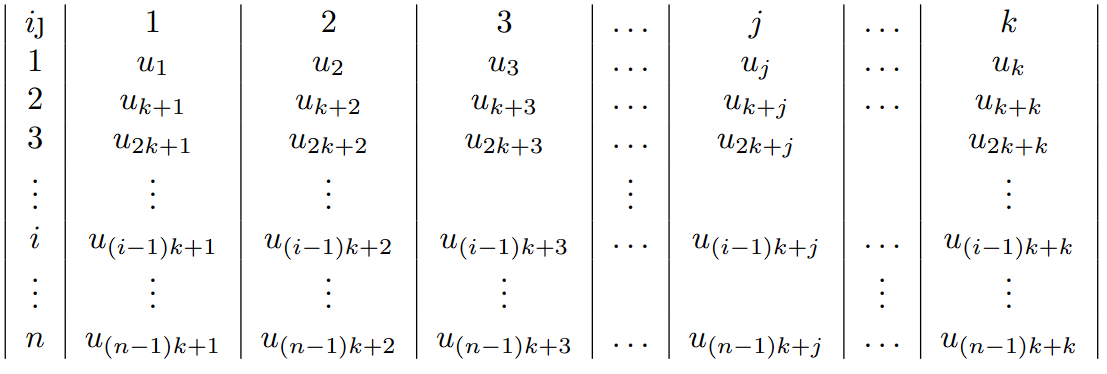
\includegraphics[scale=0.5]{img/sist.png}
    \captionof{figure}{Selección de una muestra sistemática 1 en k.}
    \label{fig:sist}
\end{center}

Una vez ordenada ya solo resta seleccionar un número aleatoriamente  entre 1 y k, el cual determinará la columna del cuadro anterior de la cual obtendremos los elementos de nuestra muestra.\\

En su traducción a un lenguaje informático, el método es muy similar. Los datos serán ordenados como una matriz, pero sin utilizar los objetos \textit{matrix}. Esto se debe a que es posible que no haya un número exacto para formar una matriz con las filas y columnas deseadas por el usuario. Este problema viene dado cuando $\frac{N}{n} = k$ no es un número entero. Para solucionar este problema, k será redondeado hacia abajo y los individuos que no completarían esa última fila de la matriz no serán seleccionados. \\

En algunos casos de la vida real, este problema llega a tener una relevancia importante, como ocurre en el método de selección de miembros a jurado popular. Para obtener estos candidatos, lo que se hace realmente es utilizar un muestreo sistemático con arranque aleatorio. Pero al realizar este tipo de selección, los electores del final de la lista tendrían probabilidad cero de ser elegidos. \\

Para evitar esta deficiencia se publicó el Real Decreto 1398/1995 artículo 3 \cite{RD}, según el cual se mantienen hasta 5 decimales del valor de k, obteniendo por lo tanto una sucesión de índices no exactos. Estos índices serán redondeados para seleccionar los individuos de una muestra que sí abarque toda la población.\\


%%Este problema ya ocurría en la vida real en el problema de selección de miembros del jurado. La solución anterior implica que los individuos situados al final de la lista censal tengan probabilidad nula de ser seleccionados para la muestra. Para evitar esto actualmente y desde la modificación del Real Decreto 1398/1995 artículo 3 \cite{RD} se mantienen hasta 5 decimales del valor de k, obteniendo por lo tanto una sucesión de índices no exactos. Estos índices serán redondeados para seleccionar los individuos de una muestra que sí abarque toda la población.\\%%

Posteriormente elegimos un número al azar entre 1 y k al que denominaremos m, y seleccionaremos los individuos con índice $m+ik, \forall i = 0,...,n-1$. De ésta forma obtenemos los individuos de la columna m siguiendo el ejemplo de la figura \ref{fig:sist}.\\

\section{Análisis de la varianza y correlación} \label{sect:5.2}
En el muestreo sistemático resulta de gran utilidad utilizar una descomposición de la información en un formato análogo al que se utiliza para el análisis de la varianza (Análysis of Variance o ANOVA) ya que nos permite obtener medidas de precisión que nos ayuden a determinar el método de estimación más preciso para nuestros datos de entre los posibles. \\

La tabla ANOVA poblacional para el análisis sistemático contiene los siguientes valores:\\

\begin{table}[H]
\centering

\begin{tabular}{|c|c|c|c|}
\hline
Fuente de variación & \begin{tabular}[c]{@{}c@{}}Grados de\\  libertad\end{tabular} & \begin{tabular}[c]{@{}c@{}}Sumas de\\ cuadrados\end{tabular}  & \begin{tabular}[c]{@{}c@{}}Cuadrados\\  medios\end{tabular} \\ \hline
Entre muestras   & $k-1$   & $\sum\limits_{i}^n\sum\limits_{j}^k(\bar{x}_j-\bar{X})^2$ & $S_{bs}^2$       \\ \hline
Intramuestras    & $N-k$   & $\sum\limits_{i}^n\sum\limits_{j}^k(X_{ij}-\bar{x}_j)^2$  & $S_{ws}^2$       \\ \hline
Total            & $N-1$   & $\sum\limits_{i}^n\sum\limits_{j}^k(X_{ij}-\bar{X})$      & $S^2$   \\ \hline        
\end{tabular}
\caption{Tabla ANOVA}
\label{tab:anova}
\end{table}

Donde $S_{bs}^2$ es la cuasivarianza intermuestral definida por:\\
\begin{equation}
    \frac{\sum\limits_{i}^n\sum\limits_{j}^k(\bar{x}_j-\bar{X})^2}{k-1}
\end{equation}

Y $S_{ws}^2$ la cuasivarianza intramuestral:\\

\begin{equation}
    \frac{\sum\limits_{i}^n\sum\limits_{j}^k(X_{ij}-\bar{x}_j)^2}{N-k}
\end{equation}

Pudiendo escribir la siguiente igualdad:\\

\begin{equation}
    (N-1)S^2 = (N-k)S_{bs}^2 + (k-1)S_{ws}^2
\end{equation}

La comparación de la cuasivarianza intermuestral e intramuestral con la cuasivarianza poblacional nos permite realizar una comparación de los distintos tipos de muestreo vistos hasta ahora. \\

Si $S_{bs}^2 > S^2$ entonces el muestreo sistemático será más preciso que el muestreo estratificado. De la misma forma si $S_{ws}^2 > S^2$ el muestreo sistemático será más preciso que el aleatorio simple. A igualdad de cuasivarianzas la precisión será la misma en ambos tipos de muestreo.\\

Otras medidas de comparación son los coeficientes de correlación intramuestral e intermuestral. Se define el primero como:\\

\begin{equation}
    \rho_{w} = \frac{2\sum\limits_j^k\sum\limits_{i<z}^n(X_{ij}-\bar{X})(X_{zj}-\bar{X})}{N(n-1)\sigma^2}
\end{equation}

 que obtiene la precisión mínima con valor 1 y precisión máxima con valor $\frac{-1}{n-1}$.\\
 
 Con $\rho_w = 0$ la precisión del muestreo sistemático coincide con el aleatorio simple con reposición. Entre este valor y 1 el muestreo aleatorio simple será más preciso que el sistemático. Valores menores que 0 hasta el valor de varianza mínima suponen el caso contrario.\\

 El coeficiente de correlación intermuestral viene dado por la expresión:
 
\begin{equation}
    \rho_{wst} = \frac{2\sum\limits_j^k\sum\limits_{i<z}^n(X_{ij}-\bar{X_i})(X_{zj}-\bar{X_z})}{n(n-1)(k-1)S_{wst}^2}
\end{equation}

 que obtiene sus valores de precisión mínima y máxima de la misma forma que con la correlación intramuestral y con la misma interpretación de sus valores permite comparar la precisión entre el muestreo sistemático y el muestreo estratificado.


\section{Estimadores lineales insesgados} \label{sect:5.3}

Sustituyendo en la fórmula general para una muestra sistemática, obtenemos los estimadores lineales insesgados en el muestreo sistemático:

\begin{equation}
    \hat{\theta} = \hat{X} = \sum_{i=1}^{n}\sum_{j=1}^1\frac{X_{ij}}{\frac{1}{k}} = \sum_{i=1}^{n}kX_{ij} = N\frac{1}{n}\sum_{i=1}^{n}X_{ij} = N\bar{x_j}
\end{equation}

\begin{equation}
    \hat{\theta} = \hat{\bar{X}} = \sum_{i=1}^{n}\sum_{j=1}^1\frac{\frac{X_{ij}}{N}}{\frac{1}{k}} = \frac{1}{n}\sum_{i=1}^{n}X_{ij} = \bar{x_j}
\end{equation}

\begin{equation}
    \hat{\theta} = \hat{P} =  \sum_{i=1}^{n}\sum_{j=1}^1\frac{\frac{A_{ij}}{N}}{\frac{1}{k}} = \frac{1}{n}\sum_{i=1}^{n}A_{ij} = \bar{P_j}
\end{equation}

\begin{equation}
    \hat{\theta} = \hat{A}  = \sum_{i=1}^{n}\sum_{j=1}^1\frac{A_{ij}}{\frac{1}{k}} = N\frac{1}{n}\sum_{i=1}^{n}A_{ij} = N\bar{P_j}
\end{equation}

\section{Estimadores de la varianza} \label{sect:5.4}
La estimación de la varianza es uno de los mayores problemas del muestreo sistemático. Al no tener un método directo, disponemos de 3 métodos de estimación diferentes con distintos resultados. En el apartado \ref{sect:6.2} vimos cómo, a partir de los valores de cuasivarianzas y correlaciones, se puede saber qué tipo de muestreo es más preciso.
Diferenciamos 3 casos:\\

\textbf{$\bullet$ \boldmath$\rho_w$ próximo a 0}\\

En el caso de $\rho_w$ positivo y próximo a 0 podemos suponer que la población está ordenada de forma aleatoria, por lo que podremos estimar la varianza con las fórmulas de muestreo aleatorio simple sobre nuestra muestra sistemática.\\

\textbf{$\bullet$ \boldmath$\rho_{wst}$ próximo a 0}\\

Para valores positivos próximos a 0 de $\rho_{wst}$ se puede considerar la falta de aleatoriedad en la selección de la muestra sobre cada zona sistemática (fila) de nuestra matriz de población. Por ello la varianza se estima tomando cada fila como un estrato y realizando las estimaciones sobre una muestra estratificada con una unidad por estrato.\\

En la práctica se supone un estrato cada 2 zonas sistemáticas, teniendo en la muestra $\frac{n}{2}$ estratos de 2 individuos por estrato. En los casos en los que $\frac{n}{2}$ no sea un número entero se repite un individuo al azar de la muestra al final para cuadrar los resultados.\\

\textbf{$\bullet$ Ni \boldmath$\rho_w$ ni \boldmath$\rho_{wst}$ próximos a 0}\\

En este caso utilizaremos el método de las muestras interpenetrantes, que se utiliza para formar un estimador cuando tenemos una o más muestras elegidas con el mismo esquema de muestreo y proporcionen por sí mismas un estimador válido del parámetro con el mismo error de muestreo.\\

Para ello se indica un parámetro extra t que representa el número de arranques o submuestras que utilizaremos para la estimación. En lugar de tomar la muestra tomada originalmente de tamaño n tomaremos t submuestras sistemáticas de tamaño $\frac{n}{t}$.\\

A partir de las submuestras podemos formar estimadores de la media y el total como:

\begin{equation}
    \bar{x_c} = \frac{1}{t}\sum_1^t\bar{x_i}
\end{equation}

\begin{equation}
    x_c = \frac{1}{t}N\sum_1^t\bar{x_i}
\end{equation}

Y sus estimadores de varianzas:

\begin{equation}
    \widehat{V(\bar{x_c})} = \frac{1}{t(1-t)}\sum_1^t(\bar{x_i}^2-\bar{x_c}^2)
\end{equation}

\begin{equation}
    \widehat{V(x_c)} = \frac{1}{t(1-t)}\sum_1^t((N\bar{x_i})^2-x_c^2)
\end{equation}

\section{Aplicaciones para el muestreo sistemático de la librería samplingR}

Las funciones desarrolladas para la aplicación de los conceptos teóricos mostrados en este capítulo utilizarán el prefijo \textit{syst} como abreviación de \textit{systematic sampling}, y son las siguientes.

\begin{itemize}[label=$\bullet$]
    \item syst.sample: Dado un tamaño poblacional N y un tamaño de muestra n devuelve una muestra sistemática, comunmente denominada 1 en k. En caso de aportar un conjunto de datos devolverá los individuos de los datos que conforman la muestra. Al ser esto opcional, si no se aporta un conjunto de datos devolverá los índices de los individuos que conforman la muestra.\\

    Realiza las funciones explicadas en el apartado \ref{sect:5.1}.

    \item syst.all.samples: Función que devuelve todas las posibles muestras sistemáticas dato un tamaño de muestra n y un tamaño poblacional N.

    \item syst.anova: Obtiene una tabla de análisis de la varianza sobre los datos de la población, siguiendo el esquema comentado en la tabla \ref{tab:anova}.

    \item syst.intercorr: Realiza el cálculo del coeficiente de correlación interclase de los datos. 

    \item syst.intracorr: Realiza el cálculo del coeficiente de correlación intraclase de los datos. \\
    
    Esto permite realizar una comparación de la precisión de la estimación entre el muestreo sistemático y el muestreo aleatorio simple.\\

     Estas tres funciones abarcan los conceptos explicados en el apartado \ref{sect:5.2}.

    \item syst.estimator: Dada una muestra de datos obtiene el estimador poblacional del parámetro especificado. También calcula su varianza estimada, error de muestreo y opcionalmente su error de estimación y un intervalo de confianza si se especifica el coeficiente de confianza en el parámetro \textit{alpha}. \\

    Realiza las funciones explicadas en el apartado \ref{sect:5.3} y \ref{sect:5.4}.

    

\end{itemize}



\newpage
\chapter{Muestreo por conglomerados}
El muestreo por conglomerados considera que los M individuos de la población están a su vez agrupados en N unidades llamadas conglomerados, de forma que sean lo más heterogéneas posibles, pero lo más homogéneas posibles entre ellas, y de forma que no haya solapamiento. Se trata por tanto del caso opuesto al del muestreo estratificado\\

Por lo tanto, en este tipo de muestreo, la unidad primaria de muestreo pasa a ser el conglomerado en lugar del individuo y por lo tanto una muestra primaria de tamaño n en el muestreo por conglomerados está formada por n conglomerados compuestos por la totalidad de sus individuos (esto en el supuesto de una muestra monoetápica). Esta forma de selección de la muestra ofrece las siguientes ventajas:\\

\begin{itemize}[label=$\bullet$]
    \item No requiere de un marco muy específico y detallado ya que no necesita la información individual de los individuos de la población.
    \item Al seleccionar aleatoriamente conglomerados en lugar de elementos individuales, se reduce la cantidad de recursos necesarios para la recopilación de datos, con el consiguiente ahorro de costes.
    \item En poblaciones grandes y dispersas, el muestreo por conglomerados puede ser más factible logísticamente, ya que por el tipo de selección facilita la organización y la ejecución del estudio.
\end{itemize}

Pero también es causa de algunas de sus principales desventajas:

\begin{itemize}[label=$\bullet$]
    \item En los casos en los que la variación dentro de los conglomerados sea mayor que la variación entre los conglomerados puede resultar en una mayor variabilidad y una reducción de la precisión de las estimaciones en comparación a otras técnicas de muestreo.
    \item Su eficiencia disminuye a medida que aumenta el tamaño de los conglomerados, que es el caso en el que este tipo de muestreo es más útil.
    \item En el caso de no seleccionar unidades de muestreo correctamente se corre el riesgo de no representar correctamente a la población e introducir sesgos en la estimación.
\end{itemize}
En este capítulo se abarcará la estimación en el caso de que los estratos sean de igual tamaño o de tamaños similares. En este último caso, lo que se suele hacer es calcular el tamaño promedio de conglomerado como $\bar{M} = \frac{\sum\limits_i^nM_i}{n}$


\section{Selección de la muestra} \label{sect:6.1}
Para la selección de la muestra y la estimación de parámetros se han diferenciado los dos casos que a continuación se indica:

\begin{itemize}[label=$\bullet$]
    \item Cuando los datos de la variable a investigar están dados a nivel de conglomerados (por ejemplo total de clase, media del conglomerado, etc.).
    \item Cuando se disponen de los datos de las unidades poblacionales de los conglomerados en la muestra.
\end{itemize}




%en los que los datos están agrupados por conglomerados, en los que para conglomerado tenemos su tamaño y en la variable de interés el total o la proporción de las respuestas de los individuos de dicho conglomerado; y los datos desglosados, en los que cada individuo tiene su información de la variable de interés y el conglomerado al que pertenece. Esto se debe a que siempre que tengamos los datos no agrupados estos pueden ser agrupados mediante un procesamiento medio pero el caso contrario no es posible. De esta forma se garantiza poder realizar estimaciones independientemente de la presentación de los datos.\\


Para obtener una muestra en el primer caso basta con tomar una de tipo aleatoria simple de los datos. Al estar agrupados por conglomerado cada instancia seleccionada para la muestra se trata de un conglomerado completo.\\

Con los datos no agrupados se crea una lista con todos los conglomerados existentes en la población. Se extrae una muestra aleatoria simple de la lista de conglomerados y se toman todos los individuos cuyo conglomerado coincida con alguno de los conglomerados de la muestra.

\section{Estimadores lineales insesgados} \label{sect:6.2}
Si al extraer la muestra se utilizara una variable de apoyo $e_i$ que toma valores 1 si el conglomerado i pertenece a la muestra con probabilidad $p=\frac{n}{N}$ y 0 en caso contrario con probabilidad 1-p, tenemos que $E(e_i) = \pi_i = \frac{n}{N}$, por lo que aplicando el estimador lineal general de Horwitz-Thompson podemos estimar los parámetros para el muestreo por conglomerados sin reemplazamiento:

\begin{equation}
    \hat{X} = \frac{\sum\limits_i^n\sum\limits_j^{\bar{M}}X_{ij}}{\pi_i} = \frac{\sum\limits_i^n\sum\limits_j^{\bar{M}}X_{ij}}{\frac{N}{n}} = \frac{N}{n}\sum\limits_i^n\sum\limits_j^{\bar{M}}X_{ij} = \frac{N}{n}\sum\limits_i^nX_i
\end{equation}

\begin{equation}
    \hat{\bar{X}} = \frac{1}{n}\sum\limits_i^n\frac{1}{\bar{M}}\sum\limits_j^{\bar{M}}X_{ij} = \frac{1}{n}\sum\limits_i^n\frac{1}{\bar{M}}X_i
\end{equation}

\begin{equation}
    \hat{P} = \frac{1}{n}\sum\limits_i^n\frac{1}{\bar{M}}\sum\limits_j^{\bar{M}}A_{ij} = \frac{1}{n}\sum\limits_i^n\frac{1}{\bar{M}}A_i
\end{equation}

\begin{equation}
    \hat{A} = \frac{N}{n}\sum\limits_i^n\sum\limits_j^{\bar{M}}A_{ij} = \frac{N}{n}\sum\limits_i^nA_i
\end{equation}

Las probabilidades de inclusión en la muestra coinciden en el muestreo con reemplazamiento por lo que sus estimadores insesgados también.

\section{Estimación de varianzas} \label{sect:6.3}
Para expresar la estimación de varianzas es preciso conocer la fórmula de la varianza entre conglomerados:\\

\begin{equation}
    \hat{S_b^2} = \frac{\sum\limits_i^n\sum\limits_j^{\bar{M}}(\bar{X_i}-\bar{X})^2}{n-1}
\end{equation}

con lo que la estimación de la varianza para el muestreo por conglomerados sin reposición es:\\

\begin{equation}
    \widehat{V(X)} = N^2\bar{M}^2(1-f)\frac{\hat{S_b^2}}{n\bar{M}}
\end{equation}

\begin{equation}
    \widehat{V(\bar{X})} = (1-f)\frac{\hat{S_b^2}}{n\bar{M}}
\end{equation}

\begin{equation}
    \widehat{V(P)} = (1-f)\frac{\hat{S_b^2}}{n\bar{M}}
\end{equation}

\begin{equation}
    \widehat{V(A)} = N^2\bar{M}^2(1-f)\frac{\hat{S_b^2}}{n\bar{M}}
\end{equation}

Para el muestreo con reposición las fórmulas se mantienen salvo por el factor (1-f).

\section{Tamaño de la muestra} \label{sect:6.4}

A la hora de su aplicación práctica y llevar a cabo la investigación estadística en campo, el diseño de muestreo por conglomerados generalmente conlleva una función de costes de muestreo en su realización.\\

El cálculo del tamaño muestral implica por lo tanto un problema de optimización con la finalidad de minimizar la varianza del estimador, con restricciones impuestas por dicha función de costes, cuya resolución es compleja y suele realizarse mediante algoritmos algebraicos de optimización iterativos, por lo que quedaría fuera del alcance de los objetivos marcados en este trabajo.\\

Si eliminamos la restricción de la función de costes podemos obtener las siguientes estimaciones para un error absoluto de muestreo dado en el muestreo sin reemplazamiento:

\begin{equation}
    e = \sqrt{\widehat{V(\hat{\bar{X}})}} = \sqrt{(1-f)\frac{\hat{S_b^2}}{n\bar{M}}} \Rightarrow n = \frac{(1-f)\hat{S_b^2}}{e^2\bar{M}}
\end{equation}

\begin{equation}
    e = \sqrt{\widehat{V(\hat{X})}} = \sqrt{(1-f)\frac{N^2\bar{M}\hat{S_b^2}}{n}} \Rightarrow n = \frac{(1-f)N^2\bar{M}\hat{S_b^2}}{e^2}
\end{equation}

Si añadimos un coeficiente de confianza para relajar el cálculo tenemos:

\begin{equation}
    e = \lambda_\alpha\sqrt{\widehat{V(\hat{\bar{X}})}} = \sqrt{(1-f)\frac{\hat{S_b^2}}{n\bar{M}}} \Rightarrow n = \\lambda_\alpha^2\frac{(1-f)\hat{S_b^2}}{e^2\bar{M}}
\end{equation}

\begin{equation}
    e = \lambda_\alpha\sqrt{\widehat{V(\hat{X})}} = \sqrt{(1-f)\frac{N^2\bar{M}\hat{S_b^2}}{n}} \Rightarrow n = \frac{\lambda_\alpha^2(1-f)N^2\bar{M}\hat{S_b^2}}{e^2}
\end{equation}

Al igual que dijimos en la estimación de varianzas, cuando realicemos el muestreo con reemplazamiento será necesario eliminar el factor (1-f) de las igualdades anteriores para realizar las estimaciones correctas.

\section{Aplicaciones para el muestreo por conglomerados de la librería samplingR}

Las funciones desarrolladas para la aplicación de los conceptos teóricos mostrados en este capítulo utilizarán el prefijo \textit{cluster} como abreviación de \textit{cluster sampling}, y son las siguientes.

\begin{itemize}[label=$\bullet$]
    \item cluster.sample: Devuelve una muestra monoetápica de conglomerados para datos no agrupados, es decir, en los que se tiene los datos de cada individuo para cada conglomerado. Dicha muestra puede ser tomada con o sin reemplazamiento, dependiendo del valor del parámetro \textit{replace}.\\

    Realiza las funciones explicadas en el apartado \ref{sect:6.1}.


    \item cluster.estimator: Dada una muestra de datos, ya sean agrupados o sin agrupar, obtiene el estimador poblacional del parámetro especificado. También calcula su varianza estimada, error de muestreo y opcionalmente su error de estimación y un intervalo de confianza si se especifica el coeficiente de confianza en el parámetro \textit{alpha}. \\

    Se permite indicar si el muestreo se realiza con o sin reemplazamiento para realizar estimaciones más precisas.\\

    Realiza las funciones explicadas en el apartado \ref{sect:6.2} y \ref{sect:6.3}.

    \item cluster.samplesize:  Calcula el tamaño de muestra necesario para cometer un error de muestreo absoluto menor del especificado. Se permite la relajación de su estimación si se especifica un coeficiente de confianza en el parámetro \textit{alpha}.\\
    
    Realiza las funciones explicadas en el apartado \ref{sect:6.4}.
\end{itemize}


\newpage
\chapter{Conclusiones y líneas futuras}
\section{Conclusiones}
En los apartado anteriores, se ha mostrado un resumen del aparato teórico que rodea a los métodos de muestreo normalmente utilizados para poblaciones finitas.\\

Como ha podido comprobarse, esos métodos se basan en una cantidad ingente de fórmulas difíciles de memorizar para poder proceder a obtener resultados de manera rápida como hoy en día demanda nuestra sociedad. Es por ello que para poder conseguir este objetivo se hace preciso ocupar un espacio hoy en día poco cubierto con herramientas informáticas. \\

En consecuencia y dada la capacidad que ofrece R para implementar técnicas estadísticas, se ha utilizado esta herramienta para implementar las técnicas que de una forma teórica se han expuesto en los apartados anteriores y además se ha hecho de una manera que sea lo más eficiente posible, tanto en la reducción del número de funciones necesarias como desde el punto de vista de la optimización del número de parámetros requeridos en esas funciones para poder conseguir el mayor número posible de estimaciones derivados de la aplicación de las mismas.\\

En resumen, desde un punto de vista informático, se ha creado una librería compuesta por 17 funciones que permiten al usuario obtener muestras, realizar estimación de parámetros sobre una muestra poblacional, calcular el tamaño muestral necesario para cometer como máximo un error de muestreo dado, realizar tablas de análisis de la varianza sobre muestras sistemáticas y obtener medidas de interés. En resumen se ha pretendido facilitar al máximo la aplicación práctica de las técnicas muestrales mostradas en apartados anteriores de este TFG\\

Estas funciones han sido creadas y diseñadas con el objetivo de minimizar el número de nombres de función que el usuario debe recordar, procurando que para la realización de una misma tarea para un tipo de muestreo determinado se deba usar siempre la misma denominación de función variando los parámetros de control de la misma.\\

La nomenclatura de las funciones está definida para poder acceder a ella de manera sencilla, empezando siempre por el tipo de muestreo con el que vayamos a trabajar (srs, strata, sys y cluster para muestreo aleatorio  simple, estratificado, sistemático y de conglomerados respectivamente) como si de un prefijo se tratara, separado por un punto del resto del nombre. Así por ejemplo tenemos que la función \textit{srs.sample} es la indicada para tomar una muestra en el muestreo aleatorio simple.\\

Además de las funciones de uso público, también constan en la librería funciones auxiliares como aquellas destinadas a evitar la repetición de código u otras como la que muestra el mensaje de bienvenida cuando se utiliza la función \textit{library(samplingR)} para poder empezar a hacer uso de sus funciones.\\

Dada la estructura que se dispone en la creación de los paquetes de R, se ha procedido a implementar líneas ayuda durante la creación de las funciones que constituyen el paquete creado en este TFG, consiguiendo de esta manera poder obtener de forma automática un pequeño manual de uso de esta librería, el cual se puede consultar en la web proporcionada por CRAN \cite{samplingR}, documento PDF que igualmente se puede ver en el anexo que figura al final de este TFG. \\

Igualmente, a continuación del manual mencionado anteriormente, también se puede ver una \textit{vignette}  creada en este TFG con la cual se pretende que con la ayuda de un ejemplo se puedan asimilar de forma eficiente los resultados de ciertas funciones que se han desarrollado dentro del paquete creado y diseñado en ese TFG.\\

Se incluye en la bibliografía un enlace a un repositorio GitHub donde se encuentra el código creado durante este trabajo para su revisión y uso, así como este documento \cite{github}.

%!!!!!!!!!!mas conclusión si es necesario%

\section{Líneas futuras}
Como se ha podido comprobar y debido a la extensión máxima establecida y a los objetivos marcados en este TFG, se ha abarcado en el mismo hasta la técnica muestral de conglomerados monoetápica y considerando además que los conglomerados son de tamaño igual o similar, por lo que aquí se deja un campo abierto a posibles futuras líneas de actuación.\\

En consecuencia y como posibles líneas de trabajo futuras están la inclusión del muestreo por conglomerados para conglomerados de distintos tamaños, así como el muestreo bietápico por conglomerados.\\

Otra posible modificación de interés sería la implantación del método actualizado de selección de muestras en el muestreo sistemático para valores de k no enteros. \cite{RD}\\

Igualmente, cabría la posibilidad de de desarrollar fórmulas de R que faciliten los cálculos para la obtención de diversos procedimientos indirectos de estimación, como pueden los denominados métodos de la razón, o de regresión.
\newpage



\newpage
\addcontentsline{toc}{chapter}{9.\hspace{1mm} Bibliografía}
\printbibliography 



\newpage
\chapter*{Anexos}
\addcontentsline{toc}{chapter}{10.\hspace{1mm} Anexos}
En esta sección se incluyen contenidos de interés disponibles en la página web proporcionada por CRAN sobre la librería creada en este trabajo \cite{samplingRweb}, compuestos por el manual de usuario con información detallada sobre las funciones desarrolladas y una viñeta creada para ejemplificar el uso de las funciones del muestreo estratificado de cálculo del tamaño de muestra y afijación, utilizando para ello herramientas creadas en la librería generada en este TFG.

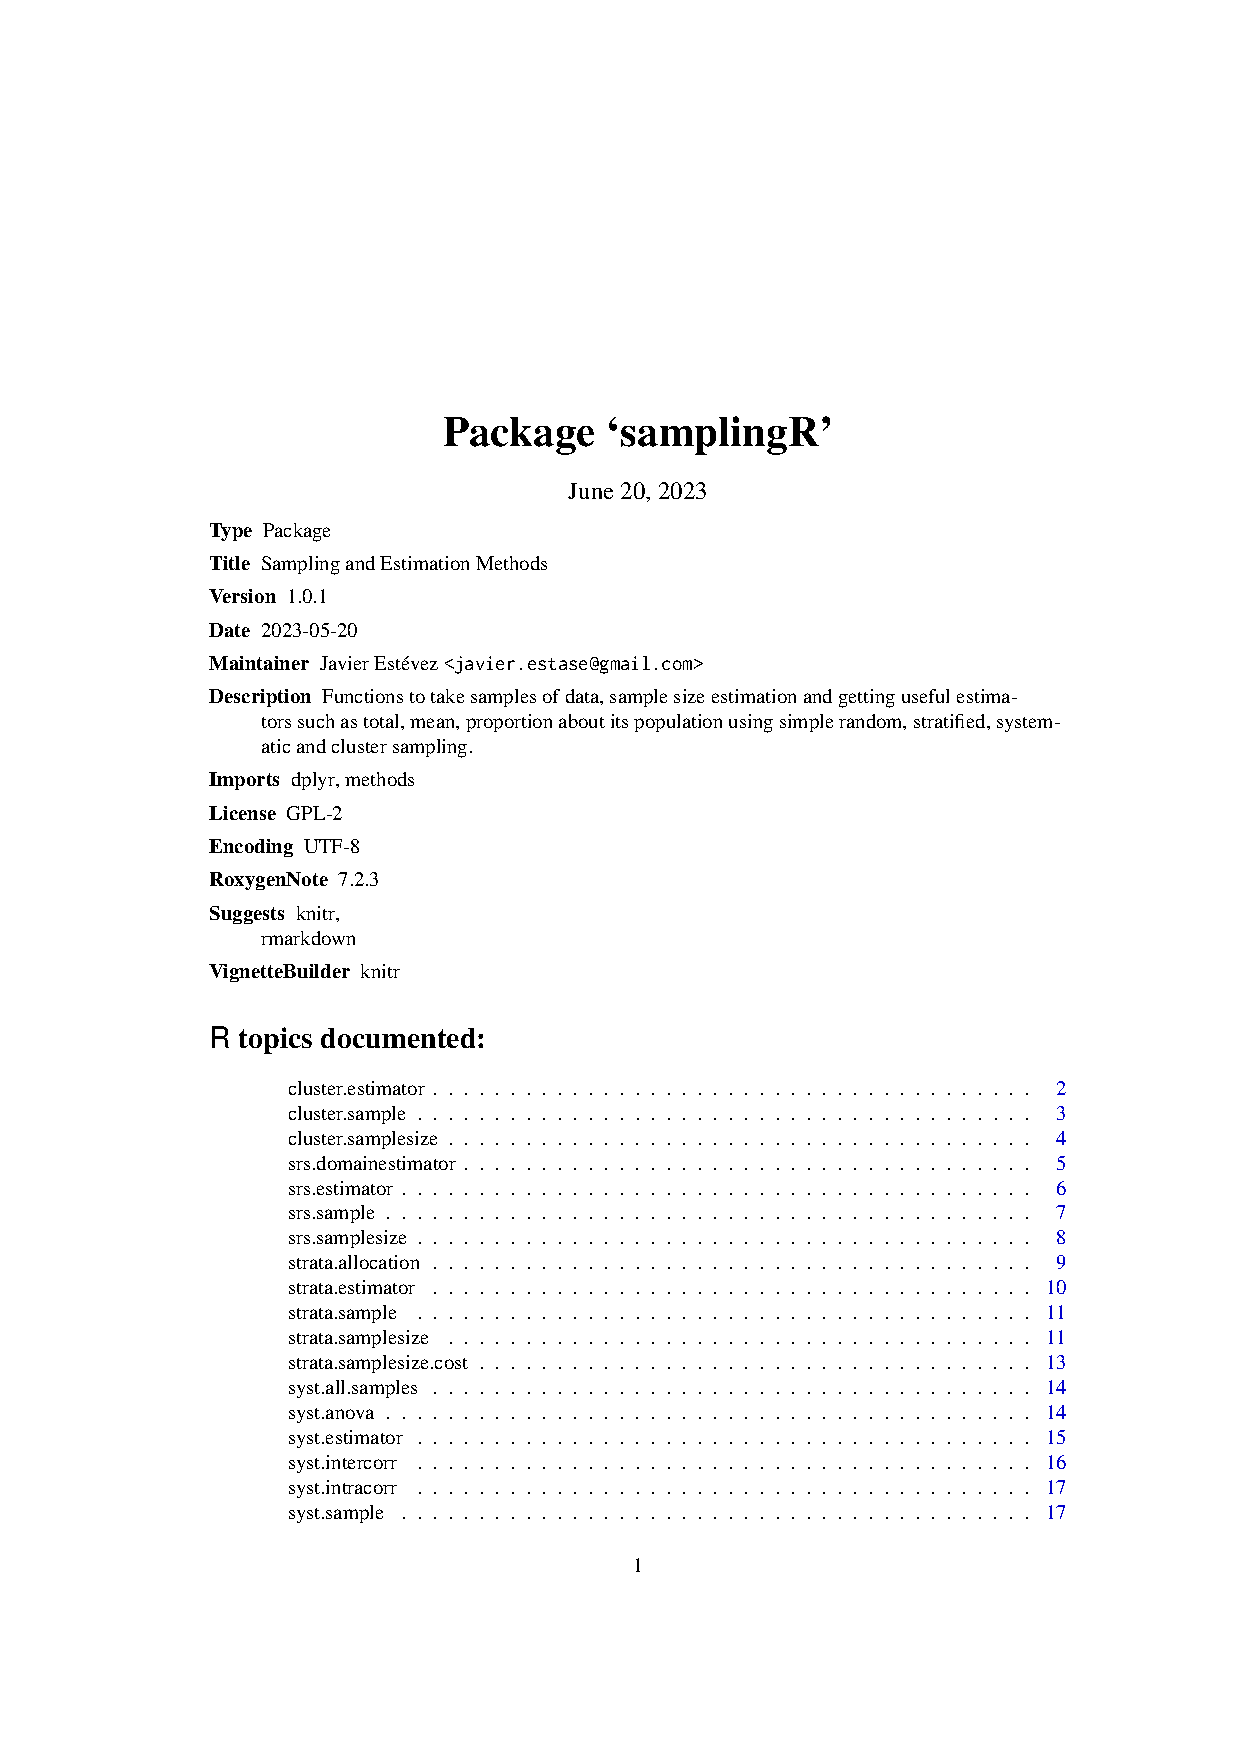
\includepdf[pages=-]{samplingR.pdf} %actualizar a la ultima version antes de subida

\label{sect:vignette}
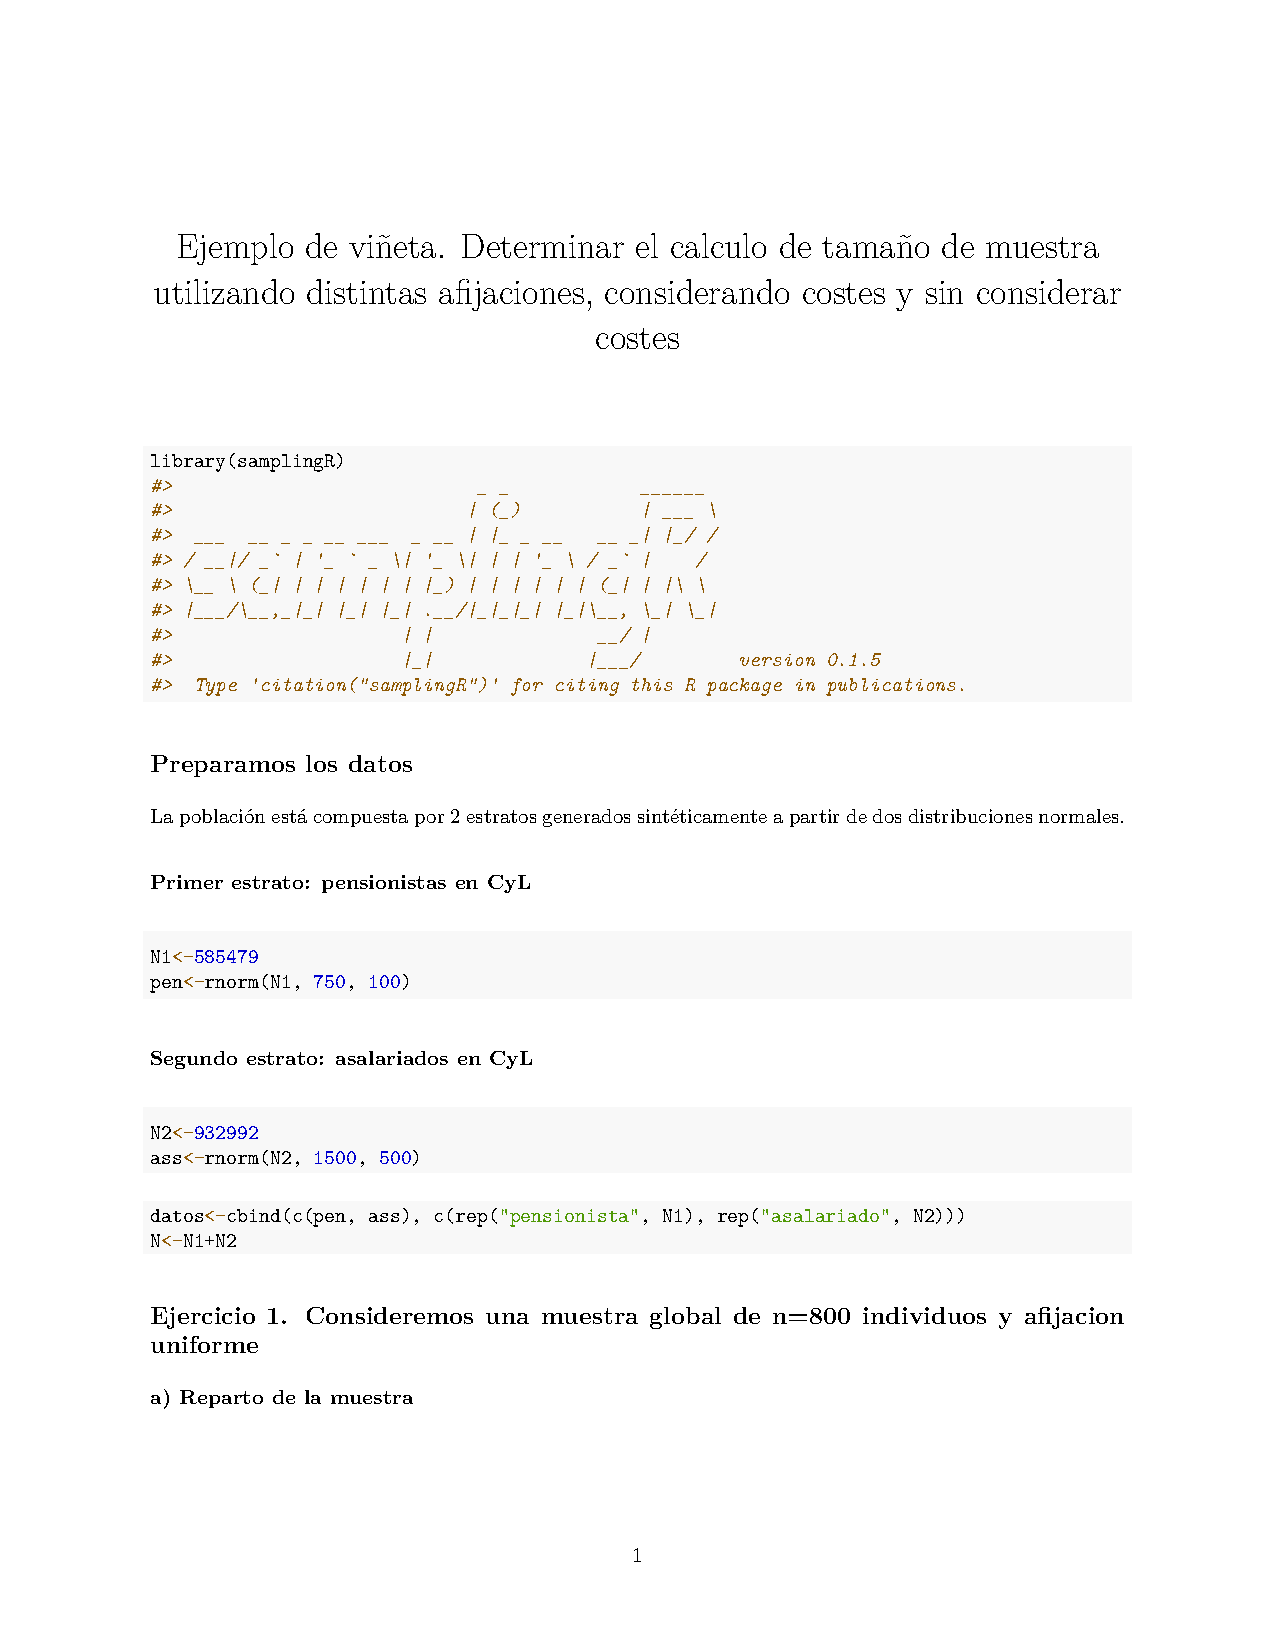
\includepdf[pages=-]{Strata.pdf}

\end{document}

